\documentclass[letterpaper,11pt]{article} % Page size, font size and document type
\usepackage[top = 2.0cm, bottom = 2.0cm, left = 2.0cm, right = 2.0cm]{geometry}

%% Encoding and language (the template was in Spanish; this report is written in English)
\usepackage[utf8]{inputenc}
\usepackage[english]{babel}
%%%%%%%%%%%%%%%%%%%%%%%%%%%%%%%%%%%%%%%%%%%%%%%%
%% Useful packages %%
\usepackage{multirow}
\usepackage{multicol}
\usepackage{booktabs}
\usepackage{graphicx}
\usepackage{setspace}
\setlength{\parindent}{0in}
\setlength{\parskip}{6pt}
\usepackage{float}
\usepackage{fancyhdr}
\usepackage{amsmath,mathtools,amsfonts,amssymb}
\usepackage[table]{xcolor} % colours for table cells
\usepackage{color}
\usepackage{fancyvrb}
\usepackage{listings}
\usepackage{enumitem}
\usepackage{tikz}
\usetikzlibrary{arrows.meta}
\usepackage{url}
\usepackage[most]{tcolorbox}
\usepackage{pgfplots}
\pgfplotsset{compat=1.17, table/col sep=comma}
\usepgfplotslibrary{groupplots,fillbetween}
\usepackage{mdframed}
\usepackage[hidelinks]{hyperref}
\usepackage{caption}

\pagestyle{fancy}
\fancyhf{}
\renewcommand{\arraystretch}{1.8}

%%%%%%%%%%%%%%%%%%%%%%%%%%%%%%%%%%%%%%%%%%%%%%%%
%% Colours
\definecolor{blond}{rgb}{0.98, 0.94, 0.75}
\definecolor{cream}{rgb}{1.0, 0.99, 0.82}
\definecolor{sunglow}{rgb}{1.0, 0.8, 0.2}
\definecolor{aliceblue}{rgb}{0.94, 0.97, 1.0}
\definecolor{cSRA}{HTML}{7F7F7F}   % SRA   = grey
\definecolor{cGBA}{HTML}{1F77B4}   % GBA   = blue
\definecolor{cABAOP}{HTML}{D62728} % ABAOP = red

%% Red marks for everything that still has to be filled in by the group
\newcommand{\todo}[1]{\textcolor{red}{\textbf{[#1]}}}

%% Box used for the Results section (same as in the template)
\newtcolorbox{Resultados}[2][]{
    enhanced,
    breakable,
    attach boxed title to top left={xshift=8mm, yshift=-3mm},
    colback=white,
    colframe=black,
    colbacktitle=white,
    coltitle=black,
    fonttitle=\ttfamily\bfseries,
    arc=4mm,
    boxrule=0.8pt,
    title={#2},
    boxed title style={
        colframe=black,
        arc=2mm,
        boxrule=0.8pt
    },
    #1
}

%% Cream frame for definitions / key statements (same as in the template)
\newmdenv[
    backgroundcolor=cream,
    linecolor=black,
    roundcorner=10pt,
    linewidth=1pt,
    topline=true,
    bottomline=true,
    leftline=true,
    rightline=true,
    innertopmargin=10pt,
    innerbottommargin=10pt,
    innerleftmargin=15pt,
    innerrightmargin=15pt,
    skipabove=10pt,
    skipbelow=10pt,
]{IOFrame}

%% Sub-titles inside the Results box (also written to the table of contents)
\newcommand{\ResSection}[1]{%
    \addcontentsline{toc}{subsubsection}{#1}%
    \par\bigskip{\Large\textbf{#1}}\par\vspace{-2mm}%
    \rule{\linewidth}{0.5pt}\par\medskip}

%% \includegraphics that does not break the compilation while an image is still missing:
%% it draws a grey box with the file name that has to be added to the folder ``figuras''.
\let\realincludegraphics\includegraphics
\renewcommand{\includegraphics}[2][]{%
  \IfFileExists{#2}%
    {\realincludegraphics[#1,height=0.4\textheight,keepaspectratio]{#2}}%
    {\fbox{\parbox[c][5.5cm][c]{0.9\linewidth}{\centering\color{gray}\ttfamily [figure to add: \detokenize{#2}]}}}}

%% Plot style shared by every pgfplots figure
\pgfplotsset{
  battle/.style={
    width=0.93\linewidth, height=6.2cm, grid=major, grid style={gray!25},
    tick label style={font=\footnotesize}, label style={font=\footnotesize}, title style={font=\footnotesize\bfseries},
    legend style={font=\scriptsize, fill=white, fill opacity=0.85, draw opacity=1, text opacity=1},
    every axis plot/.append style={line width=0.9pt}
  }
}

%%%%%%%%%%%%%%%%%% EDIT %%%%%%%%%%%%%%%%%%%%%%
\newcommand{\groupnumber}{2}
\newcommand{\semester}{2027-1}
\newcommand{\professor}{Jos\'e Jaime Camacho Escoto}
\newcommand{\studentA}{Luis Alberto Jim\'enez Rom\'an}   \newcommand{\accountA}{\todo{Account no.}}
\newcommand{\studentB}{Ram\'irez Mart\'in Edgar Alan}   \newcommand{\accountB}{\todo{Account no.}}
\newcommand{\studentC}{Gonz\'alez Falc\'on Luis Adri\'an}   \newcommand{\accountC}{\todo{Account no.}}
\newcommand{\studentD}{L\'opez Morales Fernando Samuel}   \newcommand{\accountD}{\todo{Account no.}}
\lhead{\footnotesize Artificial Intelligence 0406, Group \groupnumber}
\rhead{\footnotesize Agents for solving Battleship}
%%%%%%%%%%%%%% END EDIT %%%%%%%%%%%%%%%%%%%%%%

\cfoot{\footnotesize \thepage}
\addto\captionsenglish{\renewcommand{\refname}{Bibliography}}

%%%%%%%%%%%%%%%%%%%%%%%%%%%%%%%%%%%%%%%%%%%%%%%%
\begin{document}

\vspace*{0.2cm}
\begin{center}
    {\large\textbf{Universidad Nacional Aut\'onoma de M\'exico}}\\[1mm]
    {\large Facultad de Ingenier\'ia}\\[1mm]
    Artificial Intelligence (0406) \quad $|$ \quad Semester \semester\\[6mm]
    {\Huge\bfseries Agents for Solving the Battleship Puzzle}\\[3mm]
    {\large A comparative study of a simple reflex agent, a goal-based agent\\ and an agent based on achieving optimal performance}\\[6mm]
    \renewcommand{\arraystretch}{1.5}
    \begin{tabular}{cc}
        \studentA & \studentB \\
        \studentC & \studentD \\
    \end{tabular}\\[3mm]
    Professor: \professor \qquad Delivery date: \today
\end{center}
\renewcommand{\arraystretch}{1.8}

\vspace{2mm}
\section*{Abstract}
\addcontentsline{toc}{section}{Abstract}

Battleship is a search problem under partial observability: an agent has to locate a hidden fleet using as few shots as possible.
In this work we designed, implemented and compared three agents written in JavaScript: a Simple Reflex Agent (SRA) that shoots at random,
a Goal-Based Agent (GBA) that combines a parity-restricted search with a directed sinking routine, and an Agent Based on Achieving Optimal
Performance (ABAOP) that always fires at the cell with the highest probability density of hiding a ship.
The agents live inside a responsive web application (HTML, CSS and JavaScript, hosted on GitHub Pages) where a person can play against any of them,
watch two agents play step by step, or run thousands of games in a fast statistics mode.
Seven contests of 10\,000 games each (70\,000 games) were simulated: every pair of agents plus SRA against SRA on different fleet layouts.
Since the two agents never interact, every game is a race; to compare them fairly we used the same fleet layout for both, alternated the first shooter and let the loser finish its game.
The SRA needed $95.38\pm4.84$ shots on average, in agreement with the closed-form value of 95.39 that we derive; the GBA needed $50.29\pm8.67$ and the ABAOP $44.71\pm9.19$.
The ABAOP won 67.0\,\% of its games against the GBA (5.4 shots fewer per game, 95\,\% CI $\pm0.24$), while the SRA won only 1 of 20\,000 games against the two stronger agents.
This advantage costs computation: the ABAOP is about 53 times more expensive per shot than the SRA, although a whole game still takes only about 3 ms of CPU.
We conclude that the ABAOP is the best agent in performance, the GBA offers the best balance between cost and quality, and the SRA is useful mainly as a baseline.

\vspace{4mm}
\tableofcontents
\newpage

%%%%%%%%%%%%%%%%%%%%%%%%%%%%%%%%%%%%%%%%%%%%%%%%
\section{Goals}

The general goal of the project is to formulate, implement and compare three kinds of intelligent agents that solve the puzzle of finding a hidden fleet in the game of Battleship, and to obtain enough experimental evidence to say which one is better and at what price.
The specific goals are:

\begin{itemize}
    \item To formulate and create three different kinds of agents:
    \begin{itemize}
        \item \textbf{SRA:} Simple Reflex Agent.
        \item \textbf{GBA:} Goal-Based Agent.
        \item \textbf{ABAOP:} Agent Based on Achieving Optimal Performance.
    \end{itemize}
    \item To test the behaviour of each agent against agents of the same and of a different kind.
    \item To build an application that lets anybody use it, also from a phone, where the choices of the agents can be seen graphically and where the time between moves, or even each single step, can be controlled.
    \item To obtain statistics about the agents (number of wins, shots, hit rate and other factors) from a large number of games, so that conclusions are based on data and not on impressions.
    \item To validate the simulation against theory, and to study the computational cost of each agent through a complexity analysis.
\end{itemize}

%%%%%%%%%%%%%%%%%%%%%%%%%%%%%%%%%%%%%%%%%%%%%%%%
\section{Introduction}

Battleship looks like a game of luck, but it hides a nice problem for artificial intelligence: the agent cannot see where the ships are, it only receives a small piece of information after every shot, and it has to decide the next shot so that the whole fleet is found in as few moves as possible.
Because of that, the game has been used many times to test search and decision strategies, from simple rules to probabilistic methods \cite{berry2011,schwartz2022,vsauce2019}.
In this section we describe the rules we implemented, the framework of intelligent agents that we use to organise the three solutions and, finally, the algorithm of each agent.

%-----------------------------------------------------------------
\subsection{The basic rules of Battleship}

Battleship is a classic two-player game that was originally played with pen and paper.
Each player hides a fleet on a $10\times10$ grid, placing the ships horizontally or vertically (never diagonally) and without overlapping them; the ships may touch each other \cite{berry2011}.
The players then take turns saying a coordinate, and the opponent answers \emph{hit} if the cell belongs to a ship, \emph{miss} if it is water, and additionally announces \emph{sunk} when the last unhit cell of a ship has been hit.
The first player who sinks the whole fleet wins.
We use the standard fleet of Table~\ref{tab:fleet}: 17 ship cells hidden among 100 cells.

\begin{table}[H]
    \centering
    \renewcommand{\arraystretch}{1.4}
    \begin{tabular}{|l|c|c|}
        \hline
        \rowcolor{blue!20}
        Ship & Length (cells) & Symbol in the program \\ \hline
        Aircraft carrier & 5 & \texttt{A} \\ \hline
        Battleship & 4 & \texttt{B} \\ \hline
        Submarine & 3 & \texttt{S} \\ \hline
        Cruiser & 3 & \texttt{C} \\ \hline
        Destroyer & 2 & \texttt{D} \\ \hline
    \end{tabular}
    \caption{Standard fleet used in this work: 17 ship cells over 100 board cells.}
    \label{tab:fleet}
\end{table}

\begin{IOFrame}
\textbf{Rules as implemented.} The board is a $10\times10$ grid with rows \texttt{A}--\texttt{J} and columns 1--10. After every shot the agent learns whether it was a hit or a miss, and it is told when a ship has been sunk. Ships never overlap but may touch. A player wins when every ship of its board has been sunk.
\end{IOFrame}

In our platform, however, the two players do not shoot at each other: \emph{each agent shoots at its own board}, which holds a randomly generated fleet, and both agents play in turns.
The winner is the agent that sinks its whole fleet first, so a game is a \emph{race} between two independent runs.
This design keeps the agents completely independent, which will be very useful later to design the experiments (Section~\ref{sec:design}).

% FIGURE TODO (fig_fleet_board.png): A 10x10 board with row letters A-J and column numbers 1-10 showing the five ships in five different colours
% (lengths 5, 4, 3, 3, 2), two of them touching. Next to it (or below) the same board partly played: grey crosses for misses, red squares for hits
% and one ship completely hit (sunk) in a darker colour, so the reader understands hit / miss / sunk.
\begin{center}
    \begin{minipage}{0.9\textwidth}
        \centering
        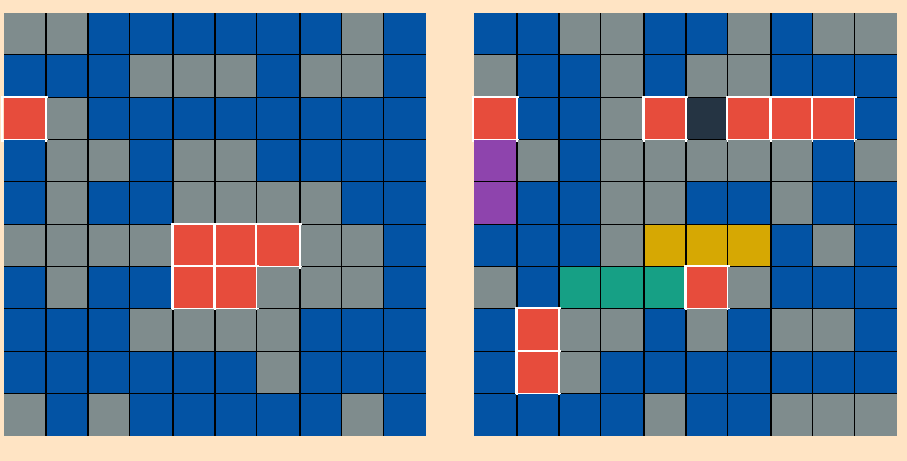
\includegraphics[width=\linewidth]{figuras/fig_fleet_board.png}
        \captionof{figure}{The Battleship board: hidden fleet (left) and a game in progress with hits, misses and a sunk ship (right).}
        \label{fig:fleet}
    \end{minipage}
\end{center}

%-----------------------------------------------------------------
\subsection{Intelligent agents}

In artificial intelligence an \emph{agent} is anything that perceives its environment through sensors and acts on it through actuators, and the way we describe a problem is through its task environment: Performance measure, Environment, Actuators and Sensors (PEAS) \cite{russell2021}.
Table~\ref{tab:peas} describes the Battleship problem in that way.

\begin{table}[H]
    \centering
    \renewcommand{\arraystretch}{1.4}
    \begin{tabular}{|l|p{12.2cm}|}
        \hline
        \rowcolor{blue!20}
        PEAS & Description in Battleship \\ \hline
        Performance measure & Number of shots needed to sink the whole fleet (fewer is better); as a consequence, winning the race; secondarily, computation time. \\ \hline
        Environment & A $10\times10$ grid with a hidden fleet of five ships (17 cells). Partially observable, discrete, static, sequential, and single-agent in our platform because the two boards do not interact. \\ \hline
        Actuators & The choice of one cell of the grid to fire at (for example \texttt{C7}). \\ \hline
        Sensors & The result of every shot (hit or miss) and the notice that a ship has been sunk. \\ \hline
    \end{tabular}
    \caption{PEAS description of the task environment.}
    \label{tab:peas}
\end{table}

Russell and Norvig \cite{russell2021} classify agents by the way they choose actions, and the three agents of this project follow that classification (Table~\ref{tab:agenttypes}):

\begin{itemize}
    \item A \textbf{simple reflex agent} selects its action from the current percept using condition--action rules.
    \item A \textbf{goal-based agent} keeps an internal state of the world and chooses actions that bring it closer to an explicit goal.
    \item A \textbf{utility-based agent}, which the course calls an \emph{agent based on achieving optimal performance}, chooses the action that maximises a performance measure (or an expected utility).
\end{itemize}

\begin{table}[H]
    \centering
    \renewcommand{\arraystretch}{1.4}
    \begin{tabular}{|c|c|p{4.2cm}|p{6cm}|}
        \hline
        \rowcolor{blue!20}
        Agent & Type & Internal state & Decision rule \\ \hline
        SRA & Simple reflex & Only the cells already shot, to avoid repeating a shot. & Fire at a cell chosen uniformly at random among the cells not shot yet. \\ \hline
        GBA & Goal based & Ships still afloat, hits not yet resolved, current mode (hunt or target), direction being explored. & Goal ``sink the ship found'': explore its neighbours in a fixed order; otherwise search only the cells of the parity class of the smallest ship afloat. \\ \hline
        ABAOP & Utility based & Complete knowledge of hits, misses, sunk ships and ships afloat. & Fire at the cell with the largest probability density of hiding a ship, recomputed after every shot. \\ \hline
    \end{tabular}
    \caption{The three agents and the kind of agent they represent.}
    \label{tab:agenttypes}
\end{table}

A remark on the SRA: a \emph{pure} reflex agent has no memory. Ours only remembers which cells were already shot (a part of the board, which is the percept history), but the \emph{results} of the shots never influence its next decision, so it behaves as a reflex agent.

% FIGURE TODO (fig_agent_types.png): Three small block diagrams side by side in the style of Russell & Norvig, one for each agent type.
% (a) Simple reflex: Sensors -> "What the world is like now" -> Condition-action rules -> Actuators, all inside the AGENT box, and the ENVIRONMENT box outside.
% (b) Goal based: adds the "State" block (how the world evolves / what my actions do) and a "Goals" block feeding "What action I should do now".
% (c) Utility based: adds a "Utility: how happy I will be in such a state" block. Label each block with the Battleship equivalent (board, shots, parity, density map).
\begin{center}
    \begin{minipage}{0.95\textwidth}
        \centering
        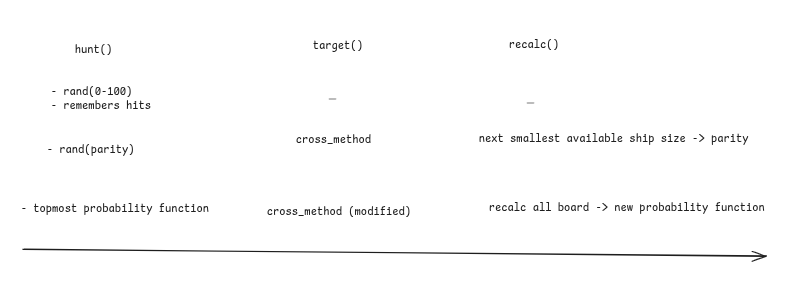
\includegraphics[width=\linewidth]{figuras/fig_agent_types.png}
        \captionof{figure}{Architecture of the three kinds of agents and its Battleship equivalent: (a) simple reflex, (b) goal based, (c) utility based.}
        \label{fig:agenttypes}
    \end{minipage}
\end{center}

%-----------------------------------------------------------------
\subsection{The algorithms}

Before describing the agents we need two words that are used in every strategy \cite{berry2011}: in \textbf{hunt} mode nothing is known about any ship still to be found, so the agent has to search; in \textbf{target} mode there is a hit on a ship that has not been sunk yet, so the agent concentrates its shots around that hit.
In the program this is the \texttt{status} of the agent, \texttt{HUNT} or \texttt{TARGET}.

\subsubsection{Simple Reflex Agent (SRA)}

The SRA does not use any knowledge about the game: at every turn it fires at a cell chosen uniformly at random among the cells that have not been shot.
If $U$ is that set of cells, the probability of choosing a particular cell $c\in U$ is
\begin{equation}
    P(c)=\frac{1}{|U|}.
\end{equation}
Its behaviour can be studied in closed form.
Let $N=100$ be the number of cells and $K=17$ the number of ship cells. Since the SRA visits the cells in a uniformly random order, the game ends at the shot $X$ in which the \emph{last} ship cell is visited.
The event $\{X\le m\}$ means that the $K$ ship cells are among the first $m$ visited cells, so
\begin{equation}
    P(X\le m)=\frac{\binom{m}{K}}{\binom{N}{K}},\qquad
    P(X=m)=\frac{\binom{m-1}{K-1}}{\binom{N}{K}},\qquad m=K,\dots,N.
    \label{eq:sra_pmf}
\end{equation}
From this distribution,
\begin{equation}
    E[X]=\frac{K(N+1)}{K+1}=\frac{17\cdot101}{18}=95.39,\qquad
    \operatorname{Var}[X]=\frac{K(N-K)(N+1)}{(K+1)^2(K+2)}=23.15\;\Rightarrow\;\sigma_X=4.81.
    \label{eq:sra_moments}
\end{equation}
Two consequences are worth noticing: the expected number of shots is almost the whole board, and the result does not depend on \emph{where} the ships are, only on $K$ and $N$. We will use Eq.~\eqref{eq:sra_pmf} in Section~\ref{sec:results} to validate the simulator.
For instance, the probability that all 100 shots are needed is $P(X=100)=K/N=17\,\%$, which agrees with the value reported in \cite{berry2011}.

% FIGURE TODO (fig_sra_random.png): A 10x10 board partly shot (about 20 cells marked with grey crosses / red hits). All the still-unshot cells are drawn with the
% same neutral colour and a caption-like label "equal probability 1/|U|". One of them is highlighted with a red frame as "randomly chosen next shot",
% and a small die icon or arrow pointing at the set of unshot cells. It must make clear that the choice ignores the previous results.
\begin{center}
    \begin{minipage}{0.7\textwidth}
        \centering
        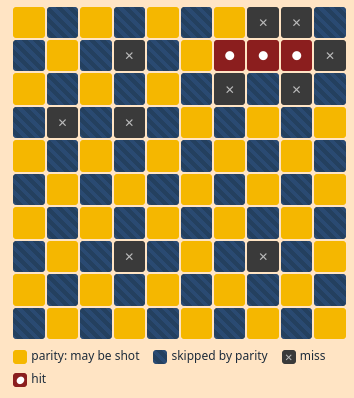
\includegraphics[width=\linewidth]{figuras/fig_sra_random.png}
        \captionof{figure}{Random choice of the SRA: every cell not shot yet has the same probability $1/|U|$ of being selected.}
        \label{fig:sra}
    \end{minipage}
\end{center}

\subsubsection{Goal-Based Agent (GBA)}

The goal of the GBA is ``sink the ship that has just been found and then find the next one''.
It keeps an internal state (ships afloat, unresolved hits, mode, direction being explored) and works in the following way.

\begin{enumerate}[label=\textbf{\arabic*.}]
    \item \textbf{Hunt with parity.} Let $p$ be the length of the shortest ship afloat. The agent only shoots at random among the not-yet-shot cells of the class
    \begin{equation}
        C_p=\{(r,c)\;:\;(r-c)\bmod p=0\}.
    \end{equation}
    This is safe because a ship of length $\ge p$ covers $p$ consecutive cells of a row or a column; along them the value $r-c$ takes $p$ consecutive integer values, so exactly one of these cells belongs to $C_p$. Hence, no ship can hide from a parity search (Fig.~\ref{fig:parity}).
    \item \textbf{Change to target mode.} A hit changes the mode to \texttt{TARGET} and the hit cell becomes the \emph{origin} $o$.
    \item \textbf{Explore the neighbours.} From the origin the agent tries \textbf{Up, Right, Down, Left}, in that order. A neighbour that is outside the board or was already shot is skipped without spending a shot.
    \item \textbf{Lock the axis.} The first hit found in a direction $d$ tells that the ship lies on that line, so the order becomes $d$, opposite of $d$, and the two perpendicular directions. The agent keeps firing in direction $d$ from its last hit until it finds a miss or the edge; then it goes back to the origin and explores the opposite direction (Fig.~\ref{fig:target}).
    \item \textbf{Ship sunk.} The ship is removed from the fleet, the parity $p$ and the class $C_p$ are recomputed with the new shortest ship, and the state of the exploration is reset. If some hit of another ship that is still afloat has an unshot neighbour (ships that touch each other), the agent goes to target mode with that hit as the new origin; otherwise it goes back to hunt mode.
    \item \textbf{Safety net.} If all the directions are exhausted and the ship is not sunk, the agent looks for another unresolved hit as origin, or returns to hunt mode.
\end{enumerate}

% FIGURE TODO (fig_gba_parity.png): Two 10x10 boards side by side. Left: p = 2 -> the cells with (r - c) even highlighted (a checkerboard pattern) and a
% destroyer (2 cells) placed anywhere over the board, always touching one highlighted cell (draw three example positions). Right: p = 3 (after the
% destroyer was sunk) -> the cells with (r - c) mod 3 = 0 highlighted as diagonal stripes, with a 3-cell ship crossing exactly one highlighted cell.
% Title each board with the parity p and the number of cells that remain candidates (50 and 34).
\begin{center}
    \begin{minipage}{0.9\textwidth}
        \centering
        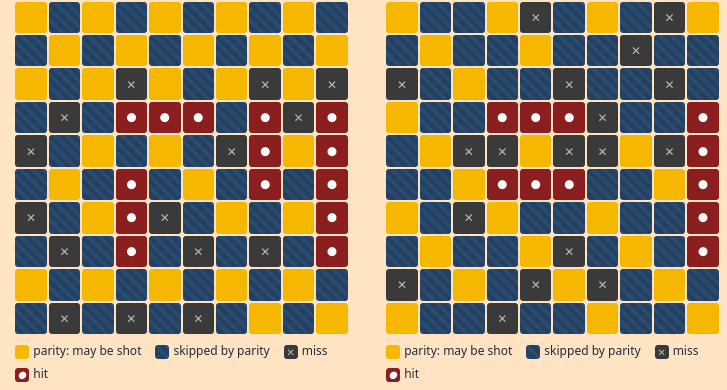
\includegraphics[width=\linewidth]{figuras/fig_gba_parity.png}
        \captionof{figure}{Parity search of the GBA: for $p=2$ (left) and $p=3$ (right), any ship of length $\ge p$ touches at least one highlighted cell, so only those cells need to be searched.}
        \label{fig:parity}
    \end{minipage}
\end{center}

% FIGURE TODO (fig_gba_target.png): Four small 7x7 board snippets in sequence (a)-(d) around a first hit (red square in the centre).
% (a) the four neighbours numbered 1-4 with arrows Up, Right, Down, Left; Up and Left are misses (grey crosses).
% (b) Right is a hit -> the axis is locked: draw a double arrow along the row and mark the new order "Right, Left, Up, Down".
% (c) the agent keeps advancing to the right until a miss appears; then a curved arrow returns to the origin.
% (d) the opposite direction (Left) is explored from the origin and the ship is completed and marked as sunk.
\begin{center}
    \begin{minipage}{0.95\textwidth}
        \centering
        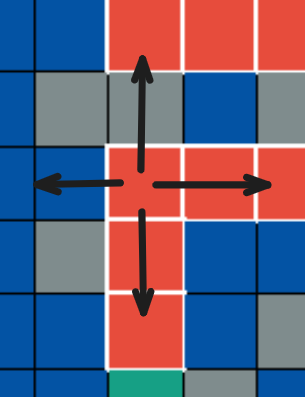
\includegraphics[width=\linewidth]{figuras/fig_gba_target.png}
        \captionof{figure}{Target mode of the GBA: exploration order Up--Right--Down--Left, locking of the axis after the first hit, advance until a miss and return to the origin to explore the opposite direction.}
        \label{fig:target}
    \end{minipage}
\end{center}

\subsubsection{Agent Based on Achieving Optimal Performance (ABAOP)}

The ABAOP builds, before every shot, a \emph{probability density map}: for every cell, how many different ways are there to hide the ships still afloat so that they cover that cell.
This is the idea described by Berry \cite{berry2011} and popularised in \cite{vsauce2019,schwartz2022}.
Let $\mathcal{F}$ be the set of ships afloat. A \emph{placement} $\pi$ is a triple (ship, orientation, position of its top-left cell), and it is \emph{legal} if the ship stays inside the board and none of its cells is a miss or a cell of a sunk ship.
For a legal placement, let $h(\pi)$ be the number of cells that are hits on ships not sunk yet. The weight of a placement is
\begin{equation}
    w(\pi)=\begin{cases}
        1 & \text{if there are no unresolved hits on the board (hunt mode)},\\
        10^{\,h(\pi)} & \text{if there are unresolved hits and } h(\pi)\ge1 \text{ (target mode)},\\
        0 & \text{if there are unresolved hits and } h(\pi)=0.
    \end{cases}
\end{equation}
The density of a cell $c$ is the sum of the weights of the placements that cover it,
\begin{equation}
    D(c)=\sum_{\substack{\pi \text{ legal}\\ c\in\pi}} w(\pi),
    \qquad
    c^{*}=\arg\max_{c\ \text{not shot}} D(c),
\end{equation}
and the agent fires at $c^{*}$, breaking ties uniformly at random. The map is recomputed after every shot.
Three comments help to understand this rule:

\begin{itemize}
    \item For a single destroyer on an empty board, a corner cell is covered by 2 placements, an edge cell by 3 and an interior cell by 4. With the whole fleet, the centre of the board gets the highest density, so the agent starts shooting at the centre.
    \item In target mode the placements that explain no hit are discarded and those that cover several hits weigh $10^{h}$ times more. This produces, without any explicit rule, the behaviour that the GBA has to be told: after one hit the neighbours are the best cells, and after two aligned hits the cells that extend the line are far better than any other. When a direction is blocked by a miss or by the edge, the placements that use it disappear and the agent changes direction by itself.
    \item The rule is greedy and approximate: it maximises the next hit, not the length of the whole game, and it counts the placements of every ship independently, without excluding those that would overlap other ships.
\end{itemize}

% FIGURE TODO (fig_abaop_density.png): The calculation of the density map step by step on a small example. Suggested: a 5x5 board with one miss and the destroyer (length 2) only.
% Panel (a): list of the horizontal placements with small arrows; panel (b): the vertical ones; panel (c): the resulting numbers written in every cell
% (sum of the placements) and coloured from light to dark; panel (d): the same idea on the real 10x10 board with the whole fleet as a heat map,
% where the darkest cell (the next shot) has a red frame. Use the same colour scale as the "decision grid" of the application.
\begin{center}
    \begin{minipage}{0.95\textwidth}
        \centering
        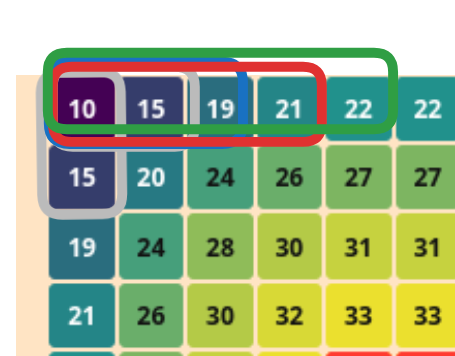
\includegraphics[width=\linewidth]{figuras/fig_abaop_density.png}
        \captionof{figure}{Calculation of the probability density of the ABAOP: every legal placement of every ship afloat adds its weight to the cells it covers; the agent shoots at the maximum.}
        \label{fig:density}
    \end{minipage}
\end{center}

%-----------------------------------------------------------------
\subsection{Related work}

Berry's analysis \cite{berry2011} simulated 100 million games for each strategy and reports, as median number of shots, 97 for random shooting, 64 for a hunt/target agent with parity and 42 for the probability-density agent; Schwartz \cite{schwartz2022} reimplemented those strategies and made the code public \cite{schwartzgit}, and the video of Vsauce2 \cite{vsauce2019} popularised the density idea.
Other videos explain the strategies to human players \cite{waytoosimple2024,always2023}.
Our SRA and ABAOP correspond directly to the random and to the density strategies of those works, while our GBA is a variation of the hunt/target strategy with a more careful sinking routine (it follows the line of the ship instead of walking around every hit).
In Section~\ref{sec:conclusions} we compare our numbers with the ones reported there.

%%%%%%%%%%%%%%%%%%%%%%%%%%%%%%%%%%%%%%%%%%%%%%%%
\section{Development}

\subsection{The application}

We wanted to create an experience that anybody can use, so we decided to build a web application.
Using only JavaScript, HTML and CSS we do not need anything more than the code and a free hosting service: the whole application is a set of static files that is published with GitHub Pages, and it runs completely in the browser of the user (there is no server).
We also thought about the experience on a phone, so the layout is responsive and the game can be played on a small screen as well.

The application has three parts (Figs.~\ref{fig:menu}--\ref{fig:phone}):

\begin{itemize}
    \item \textbf{Main menu.} The left column selects the kind of the first player and the right column the kind of the second one, among \emph{Human}, \emph{Dumb} (SRA), \emph{GBA} and \emph{ABAOP}. Only one side can be a human. When both sides are agents, the user chooses the number of games (from 1 to 10\,000) and two options: to give both agents the \emph{same fleet layout} and to \emph{alternate} the agent that shoots first. When a human plays, the number of games is fixed to one. The choice is sent to the game page through the URL (\texttt{GET} parameters \texttt{player1}, \texttt{player2}, \texttt{games}, \texttt{same\_layout} and \texttt{alternate}).
    \item \textbf{Game page.} It shows the two boards and the controls \emph{Start}, \emph{Pause/Resume}, \emph{Next move} and \emph{Stop}, together with one field $T$ (in milliseconds) for each agent, which is the delay before that agent shoots and can be changed at any moment to speed up or slow down the game. Below every board of a GBA or an ABAOP there is a button that shows its \emph{decision grid}: for the GBA, the parity cells that may be shot, the cells skipped by the parity, and the shots already made; for the ABAOP, the probability density with a colour scale and the number of every cell, with a red frame around the best cell(s). On a computer the decision grid appears below the board; on a phone it replaces the board in the same place, because two grids one over the other do not fit on the screen. The ships of the agents are drawn with one colour per ship, and hits and misses are marked on them.
    \item \textbf{Statistics mode and results.} When $T=0$ for both agents nothing is drawn and the games run at full speed. When a series ends, a panel shows the summary table and two buttons download the complete results as a JSON or a CSV file (one row per game), which are the files that we analyse in Section~\ref{sec:results}.
\end{itemize}

% FIGURE TODO (fig_app_menu.png): Screenshot of the main menu on a computer: the "Battleship" title, the two columns "Left player" / "Right player" with the four
% buttons each (one selected in yellow), the "Number of games" field and the "Play" button. If possible show the "Options" panel open.
\begin{center}
    \begin{minipage}{0.6\textwidth}
        \centering
        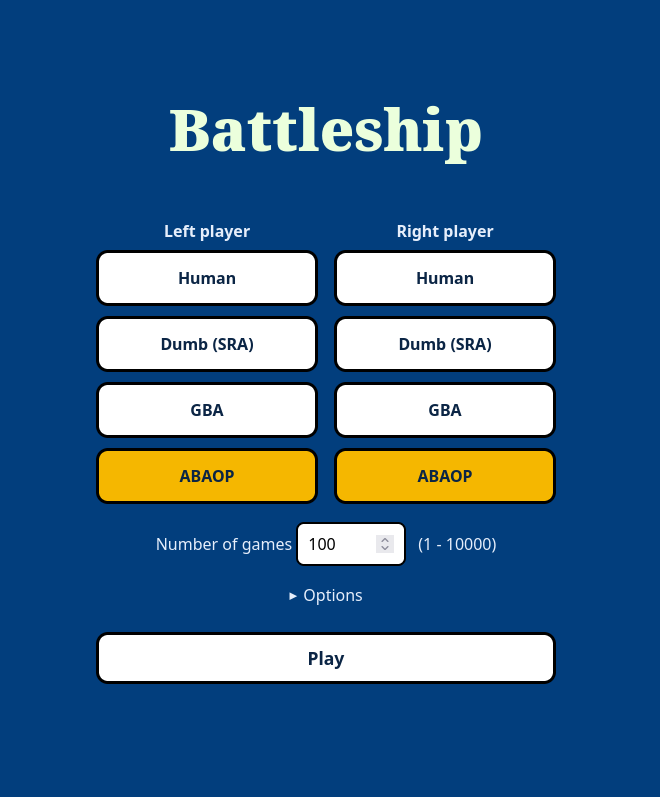
\includegraphics[width=\linewidth]{figuras/fig_app_menu.png}
        \captionof{figure}{Main menu of the application: the two columns select the kind of each player.}
        \label{fig:menu}
    \end{minipage}
\end{center}

% FIGURE TODO (fig_app_game_desktop.png): Screenshot of the game page on a computer during an ABAOP vs GBA game with the decision grid of both agents open:
% the two coloured boards on top (ships in different colours, hits with red ring, misses in grey), the two decision grids below (parity for the GBA, viridis heat map with numbers for the ABAOP),
% and the control bar at the top with Start / Pause / Next move / Stop and the two T fields.
\begin{center}
    \begin{minipage}{0.95\textwidth}
        \centering
        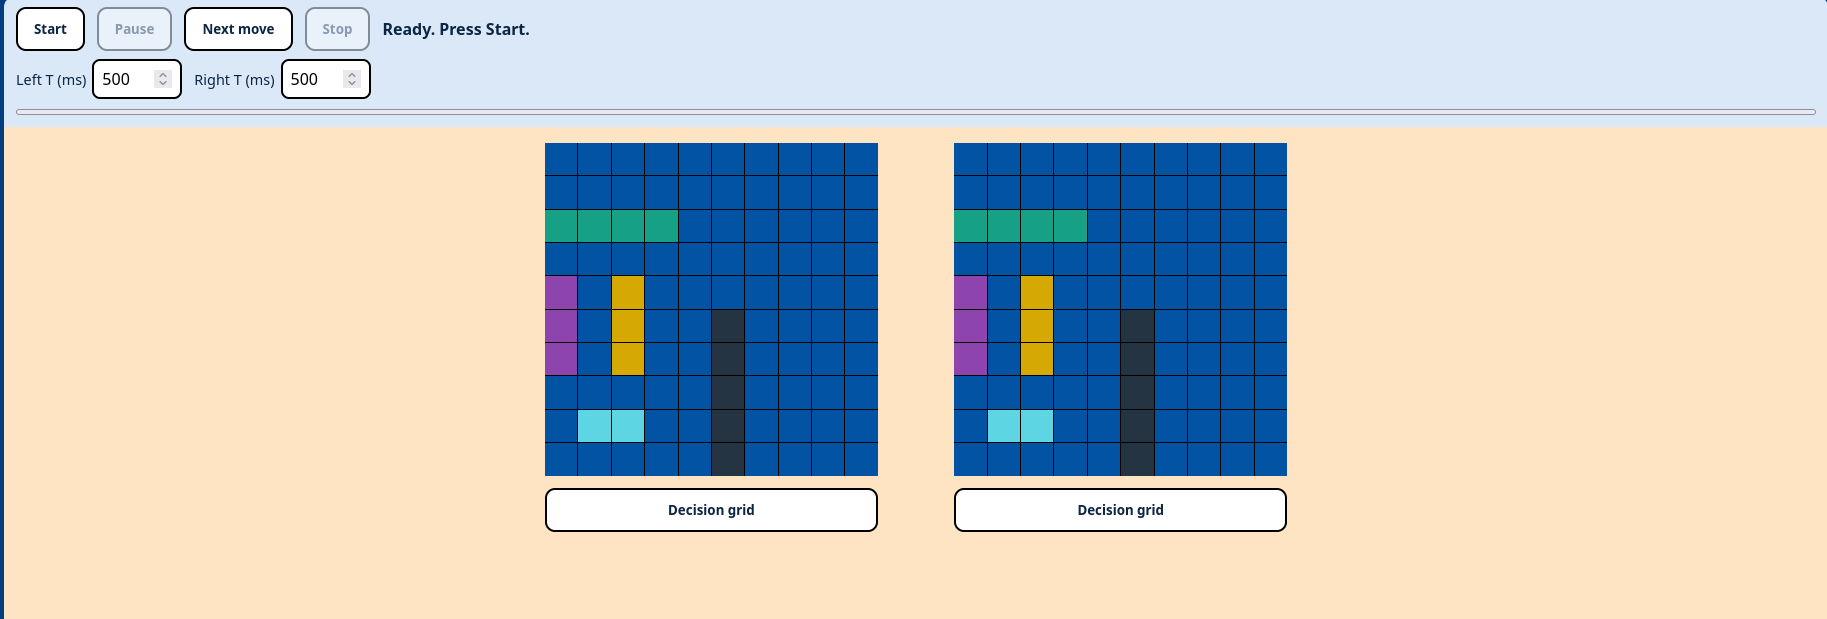
\includegraphics[width=\linewidth]{figuras/fig_app_game_desktop.png}
        \captionof{figure}{Game page on a computer: boards, control bar and decision grids of a GBA (left) and an ABAOP (right).}
        \label{fig:game}
    \end{minipage}
\end{center}

% FIGURE TODO (fig_app_phone.png): Two phone screenshots side by side (portrait). Left: the game page on a phone showing the control bar and the board.
% Right: the same page after pressing "Decision grid": the board has been replaced by the decision grid of the ABAOP (heat map with numbers).
\begin{center}
    \begin{minipage}{0.6\textwidth}
        \centering
        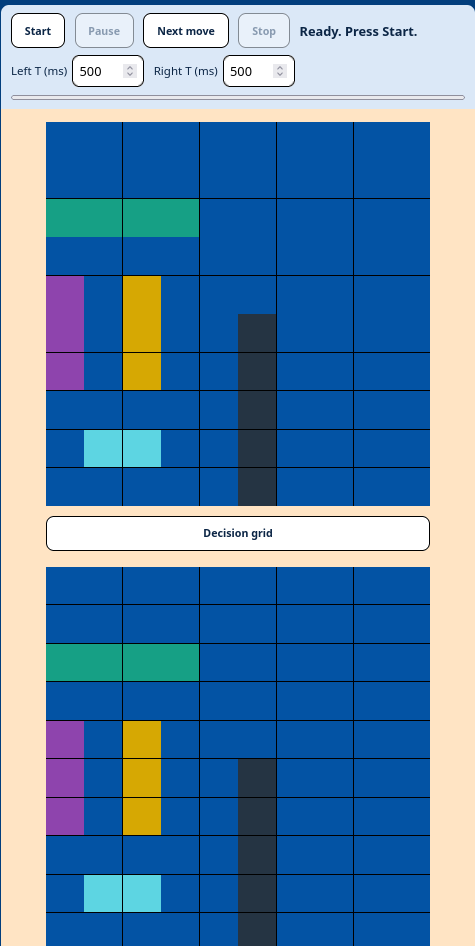
\includegraphics[width=\linewidth]{figuras/fig_app_phone.png}
        \captionof{figure}{Responsive design: on a phone the decision grid replaces the board in the same place.}
        \label{fig:phone}
    \end{minipage}
\end{center}

%-----------------------------------------------------------------
\subsection{The program}

The whole solution is implemented with Object-Oriented Programming (OOP) in JavaScript (ES2022 classes), so the functionality is directly connected to the entities of the problem.

\begin{itemize}
    \item \texttt{Battleship\_Agent} is the base class. It owns the board of the agent (a $10\times10$ matrix of characters: \texttt{o} water, an upper-case letter for a ship cell not discovered yet, the same letter in lower case for a hit, and \texttt{X} for a miss), the fleet, the conversion between coordinates such as \texttt{C7} and matrix positions, the random generation of the fleet, and the common operations \texttt{hunt}, \texttt{hit}, \texttt{miss}, \texttt{sunk}. A human player is an instance of this class that does not choose automatically.
    \item \texttt{Battleship\_SRA}, \texttt{Battleship\_GBA} and \texttt{Battleship\_ABAOP} inherit from it and override only what makes them different: how the next cell is chosen (\texttt{nextValidMove}), what happens in target mode (\texttt{target}) and what is recomputed when a ship is sunk (\texttt{recalc}).
    \item \texttt{Game} controls one match between two agents (whose turn it is, the timers, the human clicks, the end of the game) and \texttt{Series} runs many matches and collects the statistics.
    \item Two view files, one for the boards and one for the decision grids, draw the state of the agents, and a script handles the main menu.
\end{itemize}

OOP was a good choice for several reasons.
\emph{Encapsulation}: the counters and the state that must not be modified from outside (remaining cells, number of shots, delay $T$, automatic or human) are private fields of the class.
\emph{Inheritance}: the three agents share the whole logic of the board and differ only in a few methods, so a new agent can be added by writing one class.
\emph{Polymorphism}: \texttt{Game} calls \texttt{agent.step()} without knowing the kind of agent, which is what allows to combine any pair of agents, or a human, with a single piece of code.
Finally, the behaviour of every agent can be tested in isolation.

We also used the \textbf{event-oriented paradigm}, which is natural in JavaScript.
The game is not a \texttt{while} loop that blocks the page: it is a chain of events. A click on a cell of the board is an event that calls \texttt{Game.human\_shot}; a timer of $T$ milliseconds is an event that makes an agent shoot; a change in a $T$ field is an event that updates the delay of the running game; and the end of a game is an event that triggers the record of the results and the start of the next game.
JavaScript runs on a single thread with an \emph{event loop} \cite{mdnloop}, so the page never freezes while it waits, and the code that draws the boards is completely separated from the code that plays: the game only announces ``an agent has shot'' and the view, which registered itself as a listener, redraws.
This decoupling is what allows the same game logic to run with or without drawing.
Even in statistics mode, where thousands of games are played in a synchronous loop, the series releases the thread every few tens of milliseconds so that the progress bar and the buttons keep responding.

%-----------------------------------------------------------------
\subsection{Technologies used}

\begin{itemize}
    \item \textbf{JavaScript} (ES2022: classes, private fields, \texttt{async/await}) for the agents, the game logic and the statistics.
    \item \textbf{HTML5} for the structure of the menu and of the game page.
    \item \textbf{CSS3} for the appearance: CSS grid for the boards, custom properties and media queries for the responsive design.
    \item \textbf{GitHub and GitHub Pages} for version control and for publishing the application.
    \item \textbf{Python} (pandas, NumPy, SciPy) to analyse the CSV files of the experiments, and \textbf{\LaTeX} with pgfplots to write this report and draw its graphics from those data.
\end{itemize}

%-----------------------------------------------------------------
\subsection{Execution of a game}

Every agent is a small state machine. It starts in \texttt{HUNT}; a hit moves it to \texttt{TARGET}; when a ship is sunk the method \texttt{recalc} recomputes what depends on the fleet and decides whether the next mode is \texttt{TARGET} (there are hits of another ship still unresolved) or \texttt{HUNT}.
The agent that must shoot next is decided by \texttt{Game}. Its method \texttt{schedule} reads the delay $T$ of that agent \emph{at that moment} and arms a timer; when the timer fires the agent makes one shot (\texttt{step}) and \texttt{schedule} is called again. Because $T$ is read every time, a change of $T$ takes effect on the next shot. If the turn belongs to a human, \texttt{schedule} does nothing and the game waits for a click.
If both delays are zero, \texttt{Game} switches to a synchronous loop (\texttt{run\_headless}) that plays the game without timers and without drawing.
The button \emph{Next move} performs exactly one shot of the agent whose turn it is, and pauses the game, so it can be used to follow an agent step by step (Fig.~\ref{fig:flow}).

% FIGURE TODO (fig_execution_flow.png): Flowchart of the execution. Start button -> Series.run() -> new Game -> "T = 0 for both agents?" ->
% YES: run_headless (loop until one agent wins, then the loser plays out) -> record the game -> next game (no drawing, yield to the page every ~40 ms).
% NO: schedule() -> timer of T ms -> agent.step() -> redraw -> game over? (no: back to schedule; yes: record, wait ~1 s, next game).
% Show the side entries "Pause", "Next move" (one step, pauses) and "human click" (human_shot) joining the diagram.
\begin{center}
    \begin{minipage}{0.85\textwidth}
        \centering
        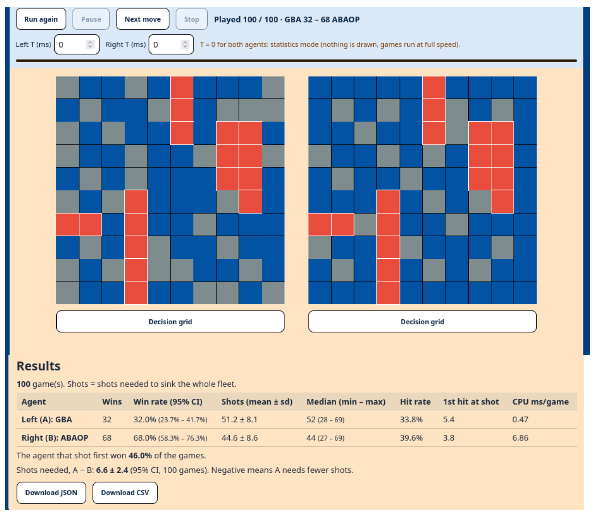
\includegraphics[width=\linewidth]{figuras/fig_execution_flow.png}
        \captionof{figure}{Execution of a series of games: timed mode (with drawing) and statistics mode ($T=0$).}
        \label{fig:flow}
    \end{minipage}
\end{center}

%-----------------------------------------------------------------
\subsection{The most important functions}

Table~\ref{tab:functions} lists the functions that concentrate the behaviour of the program.
The method \texttt{continue}, which in the first version of the program was the one that allowed the game to continue after every turn (it armed a timer inside each agent), was replaced by \texttt{Game.schedule}, because the control of the turns is a responsibility of the match and not of a single agent.

\begin{table}[H]
    \centering
    \small
    \renewcommand{\arraystretch}{1.35}
    \begin{tabular}{|l|l|p{8.2cm}|}
        \hline
        \rowcolor{blue!20}
        Function & Class & What it does \\ \hline
        \texttt{hunt(m)} & \texttt{Battleship\_Agent} & Chooses the cell (or receives it, for a human), decides hit or miss, and moves the agent to \texttt{TARGET} after a hit. \\ \hline
        \texttt{target()} & GBA, ABAOP & GBA: explores the neighbours of the hit in the order Up--Right--Down--Left, locks the axis and reverses. ABAOP: fires at the maximum of the density map. \\ \hline
        \texttt{nextValidMove()} & SRA, GBA, ABAOP & Random cell among the unshot ones (SRA), random cell of the parity class (GBA), cell of maximum density with random tie-break (ABAOP). \\ \hline
        \texttt{hit(m)}, \texttt{miss(m)} & \texttt{Battleship\_Agent} & Update the symbol of the board, count the hit for its ship, register the first hit, and detect that a ship has been sunk. \\ \hline
        \texttt{valid\_move(m)} & \texttt{Battleship\_Agent} & Counts the shot and removes the cell from the list of available cells, so no cell is shot twice. \\ \hline
        \texttt{sunk(symbol)}, \texttt{recalc()} & Base, GBA, ABAOP & Remove the ship from the fleet, test whether the agent has won, recompute the parity or the density and decide the next mode. \\ \hline
        \texttt{step()} & \texttt{Battleship\_Agent} & One automatic shot without timers: \texttt{target()} if the status is \texttt{TARGET}, \texttt{hunt()} otherwise (the SRA always hunts). \\ \hline
        \texttt{schedule()} & \texttt{Game} & Decides who shoots next and arms the timer with the current $T$ (it replaces \texttt{continue}); switches to \texttt{run\_headless} when $T=0$. \\ \hline
        \texttt{run\_headless()} & \texttt{Game} & Plays a whole game synchronously; the loser then plays out its own board so that its number of shots is not cut short. \\ \hline
        \texttt{run()}, \texttt{record()} & \texttt{Series} & Plays the games one after another without blocking the page and builds one record (row of the CSV) per game. \\ \hline
        \texttt{summarize()} & Statistics & Computes means, deviations, win rates with their intervals and the paired difference of shots. \\ \hline
        \texttt{draw\_visual\_grid()} & \texttt{Battleship\_Agent} & Paints the ships, hits and misses on the board of the page. \\ \hline
    \end{tabular}
    \caption{Main functions of the program.}
    \label{tab:functions}
\end{table}

%-----------------------------------------------------------------
\subsection{Design of the experiments}
\label{sec:design}

Seven contests of 10\,000 games each were played in statistics mode (Table~\ref{tab:contests}): the three possible pairs of different agents, the three pairs of agents of the same kind, and SRA against SRA once more but with a different random layout for each agent.
The number 10\,000 was chosen because, as will be seen, the standard error of a mean of shots is then about $0.1$ shots, and because the whole batch of the slowest contest takes about a minute.

\begin{table}[H]
    \centering
    \renewcommand{\arraystretch}{1.4}
    \begin{tabular}{|c|l|c|c|c|}
        \hline
        \rowcolor{blue!20}
        \# & Contest (left vs right) & Layout & Games & First shooter \\ \hline
        1 & SRA vs SRA & same & 10\,000 & alternates \\ \hline
        2 & SRA vs SRA & \emph{different} & 10\,000 & alternates \\ \hline
        3 & GBA vs GBA & same & 10\,000 & alternates \\ \hline
        4 & ABAOP vs ABAOP & same & 10\,000 & alternates \\ \hline
        5 & SRA vs GBA & same & 10\,000 & alternates \\ \hline
        6 & SRA vs ABAOP & same & 10\,000 & alternates \\ \hline
        7 & GBA vs ABAOP & same & 10\,000 & alternates \\ \hline
    \end{tabular}
    \caption{Contests simulated in this work (70\,000 games in total).}
    \label{tab:contests}
\end{table}

Since each agent shoots at its own board, a game is a race, and three decisions were taken to make the comparison fair:

\begin{enumerate}[label=\textbf{\arabic*.}]
    \item \textbf{Same layout (paired design).} In six contests both agents attack the same fleet layout, so the difference in their results is due to the agent and not to the luck of the layout. Contest 2 uses independent layouts on purpose, to measure what the pairing changes (subsection \emph{Effect of the fleet layout} of the Results).
    \item \textbf{The first shooter alternates.} If both agents finish in the same number of shots, the one that shoots first wins. Alternating the first shooter game by game removes that bias from the win rates, so ``ABAOP vs GBA'' and ``GBA vs ABAOP'' are the same experiment.
    \item \textbf{The loser plays out.} When the winner finishes, the loser is still allowed to finish its own board. As the agents never interact, this does not change who wins, and it gives the real number of shots that each agent needs. Without it, the shots of the loser would be truncated by the moment at which the opponent finished, and their averages would be biased downwards.
\end{enumerate}

Each game produces one record with the fields of Table~\ref{tab:fields}, and the application exports the records of a series as a CSV file.

\begin{table}[H]
    \centering
    \small
    \renewcommand{\arraystretch}{1.3}
    \begin{tabular}{|l|p{11.6cm}|}
        \hline
        \rowcolor{blue!20}
        Field (suffix \texttt{\_A} / \texttt{\_B}) & Meaning \\ \hline
        \texttt{game}, \texttt{first}, \texttt{winner} & Game number, agent that shot first and agent that won the race. \\ \hline
        \texttt{moves} & Shots taken \emph{when the game ended}. \\ \hline
        \texttt{hits}, \texttt{sunk} & Hits and ships sunk \emph{when the game ended}. \\ \hline
        \texttt{full} & Shots the agent needs to sink \emph{all} its ships (after playing out). \\ \hline
        \texttt{first\_hit} & Number of the shot that produced the first hit. \\ \hline
        \texttt{sunk\_at} & Shot number at which each of the five ships was sunk, in order. \\ \hline
        \texttt{cpu\_ms} & CPU time spent by the agent to decide all its shots, in milliseconds. \\ \hline
    \end{tabular}
    \caption{Fields of the record of a game (CSV columns).}
    \label{tab:fields}
\end{table}

\subsection{Limitations of the model}

We want to be clear about what this study does not include.
(i) It is a race on independent boards; there is no opponent who hides the ships against the strategy of the agent.
(ii) The agents know when a ship is sunk and which ship it was, as in the official rules, and the program uses the letter of a hit cell to know whether that hit belongs to a ship already sunk; a human player would deduce that from the announcement, but would sometimes have to guess which cells belong to it.
(iii) The board is always $10\times10$ with the standard fleet.
(iv) The CPU times were measured in a browser with \texttt{performance.now()}, whose resolution is intentionally coarsened by browsers \cite{mdnperf}; in our files every value is an integer number of milliseconds, so the time of one game is coarse and only averages over many games are meaningful.

%%%%%%%%%%%%%%%%%%%%%%%%%%%%%%%%%%%%%%%%%%%%%%%%
\section{Results}
\label{sec:results}

This section presents the analysis of the 70\,000 games that were simulated with the application (Table~\ref{tab:contests}).
First the statistics are defined, then the data and the simulator are validated, and after that the results are presented: shots, wins, first-shooter advantage, graphics of the contests, secondary statistics, effect of the layout and, finally, the computational cost and the complexity analysis of the three agents.

\addcontentsline{toc}{subsection}{Results and analysis}
\begin{Resultados}{Results and analysis}
\vspace{2mm}

%=========================================================================================
\ResSection{Metrics and how they were calculated}

Let $G=10\,000$ be the number of games of a contest. For game $g$ and one agent we record the following quantities (fields of Table~\ref{tab:fields}); the formulas are the ones used both by the web application and by the analysis script.

\begin{itemize}
    \item \textbf{Shots} $S_g$: number of shots the agent needs to hit the 17 ship cells, i.e. to sink the whole fleet, after playing out (so $17\le S_g\le100$). The summaries are the mean, the standard deviation, the median with the range, and the percentiles:
    \begin{equation}
        \bar S=\frac{1}{G}\sum_{g=1}^{G}S_g,\qquad s=\sqrt{\frac{1}{G-1}\sum_{g=1}^{G}\left(S_g-\bar S\right)^2},\qquad \bar S\pm1.96\,\frac{s}{\sqrt G}\ \ \text{(95\,\% CI of the mean)}.
    \end{equation}
    The median is the middle value of the sorted $S_g$, and ``min--max'' are its extremes.
    \item \textbf{Hits} $H_g$: shots that fell on a ship cell. At the end of the whole game $H_g=17$; at the moment in which the \emph{game ended} it is 17 for the winner and smaller for the loser.
    \item \textbf{Hit rate.} The application computes it \emph{per game}, at the moment in which the game ends, and then averages the games,
    \begin{equation}
        \bar h=\frac{1}{G}\sum_{g=1}^{G}\frac{H_g}{M_g},
    \end{equation}
    where $M_g$ is the number of shots fired at that moment. Because the loser is cut in the middle of its game, we also report the \emph{whole-game} hit rate, $\frac{1}{G}\sum_g 17/S_g$, which is not affected by the moment in which the opponent finished. Both are averages of per-game rates; they are not equal to $17/\bar S$.
    \item \textbf{Ships sunk} $Z_g\in\{0,\dots,5\}$: ships sunk at the moment in which the game ended (always 5 for the winner).
    \item \textbf{First hit} $F_g$: the number of the shot that produced the first hit; we report its mean and median.
    \item \textbf{When each ship sank} $T_{g,k}$: the number of the shot in which the $k$-th ship (in order of sinking) was sunk, $k=1,\dots,5$, so $T_{g,5}=S_g$. We report $\bar T_k=\frac1G\sum_g T_{g,k}$.
    \item \textbf{Win rate.} If $w$ games are won by an agent, $\hat p=w/G$, with the Wilson 95\,\% interval \cite{wilson1927}
    \begin{equation}
        \frac{\hat p+\frac{z^2}{2G}\;\pm\; z\sqrt{\frac{\hat p(1-\hat p)}{G}+\frac{z^2}{4G^2}}}{1+\frac{z^2}{G}},\qquad z=1.96.
    \end{equation}
    \item \textbf{Whether the first shooter won.} $W_g=1$ if the agent that shot first won game $g$; the rate is $\frac1G\sum_g W_g$ and its interval is also a Wilson interval.
    \item \textbf{CPU ms per game.} Sum of the times (measured with \texttt{performance.now()}) that the agent spent inside its \texttt{step()} routine during the whole game, including the play-out. We also give the time per shot, $\sum_g \text{cpu}_g / \sum_g S_g$.
\end{itemize}

\textbf{The difference in shots and its 95\,\% interval.} As both agents attack the same layout, each game gives a natural pair $(S^A_g,S^B_g)$ and we look at the paired difference
\begin{equation}
    d_g=S^A_g-S^B_g,\qquad \bar d=\frac1G\sum_g d_g,\qquad \bar d\;\pm\;1.96\,\frac{s_d}{\sqrt G}.
\end{equation}
A negative $\bar d$ means that agent A needs fewer shots. The interval says how well we know the true average difference: if the experiment were repeated many times, about 95\,\% of the intervals built in this way would contain the true difference. Two things can be read from it: its \emph{size} ($\bar d$ is the number of shots that one agent saves per game, and the half-width tells how precise that number is) and whether it contains \emph{zero}: if it does not, the difference is statistically significant at the 5\,\% level. We also report $t=\bar d/(s_d/\sqrt G)$ with its $p$-value, and the effect size $d_z=\bar d/s_d$, that compares the difference with the game-to-game noise. For agents of the same kind the true difference is zero, so their interval should contain zero.

%=========================================================================================
\ResSection{Validation of the data and of the simulator}

Before analysing the results we checked that the 70\,000 records are consistent (Table~\ref{tab:integrity}). In every game (i) the winner is the agent that finishes first, with the tie-break given to the first shooter (if $S^A<S^B$, or $S^A=S^B$ and A shot first, A wins); (ii) the last of the five sinking times equals the total number of shots; (iii) the number of shots is between 17 and 100; and there are no empty fields. All the checks are satisfied in 100\,\% of the games.

\begin{table}[H]
    \centering
    \small
    \renewcommand{\arraystretch}{1.35}
    \resizebox{\linewidth}{!}{\begin{tabular}{|l|l|c|c|c|c|}
\hline
\rowcolor{aliceblue}
Contest & File & Games & Winner = first to finish & Last ship at final shot & Shots in [17,100] \\ \hline
SRA vs SRA & \texttt{SRA-SRA\_samegrid\_.csv} & 10\,000 & 100.0\% & 100.0\% & 100.0\% \\ \hline
SRA vs SRA (diff.) & \texttt{SRA-SRA\_different\_grid\_.csv} & 10\,000 & 100.0\% & 100.0\% & 100.0\% \\ \hline
GBA vs GBA & \texttt{GBA-GBA.csv} & 10\,000 & 100.0\% & 100.0\% & 100.0\% \\ \hline
ABAOP vs ABAOP & \texttt{ABAOP-ABAOP.csv} & 10\,000 & 100.0\% & 100.0\% & 100.0\% \\ \hline
SRA vs GBA & \texttt{SRA-GBA.csv} & 10\,000 & 100.0\% & 100.0\% & 100.0\% \\ \hline
SRA vs ABAOP & \texttt{SRA-ABAOP.csv} & 10\,000 & 100.0\% & 100.0\% & 100.0\% \\ \hline
GBA vs ABAOP & \texttt{GBA-ABAOP.csv} & 10\,000 & 100.0\% & 100.0\% & 100.0\% \\ \hline
\end{tabular}
}
    \caption{Consistency checks of the data (percentage of games that satisfy each check).}
    \label{tab:integrity}
\end{table}

The SRA has a closed-form distribution (Eq.~\eqref{eq:sra_pmf}), which allows a check of the simulator against theory (Table~\ref{tab:sra_theory}). The mean, standard deviation, median, probability of needing the 100 shots and the mean shot of the first hit agree with the theory within their sampling error. A $\chi^2$ goodness-of-fit test of the distribution of the 60\,000 SRA games against Eq.~\eqref{eq:sra_pmf} gives $\chi^2=31.6$ with 36 degrees of freedom ($p=0.68$), and the largest distance between the empirical and the theoretical cumulative distributions is $0.002$; so the data are compatible with the theory and we have no evidence of a problem in the random generation of the layouts or of the shots.

\begin{table}[H]
    \centering
    \renewcommand{\arraystretch}{1.4}
    \begin{tabular}{|l|c|c|}
\hline
\rowcolor{sunglow}
Quantity & Theory (closed form) & Observed (SRA, 60\,000 games) \\ \hline
Mean shots to finish & 95.39 & 95.38 \\ \hline
SD of shots to finish & 4.81 & 4.84 \\ \hline
Median shots to finish & 97 & 97 \\ \hline
$P(\text{all 100 shots needed})$ & 17.00\% & 17.14\% \\ \hline
Mean shot of the 1st hit & 5.61 & 5.60 \\ \hline
\end{tabular}

    \caption{Simple Reflex Agent: closed-form theory (Eqs.~\eqref{eq:sra_pmf}--\eqref{eq:sra_moments} and $E[F]=(N+1)/(K+1)$ for the first hit) against the simulation.}
    \label{tab:sra_theory}
\end{table}

Finally, each agent plays independently of its opponent, so its average number of shots should be the same in every contest in which it took part. A one-way analysis of variance confirms it (SRA, 4 contests: $p=0.77$; GBA, 3 contests: $p=0.13$; ABAOP, 3 contests: $p=0.55$). Therefore, in the next sections we pool all the games of an agent to describe it (60\,000 games for the SRA, and 40\,000 for the GBA and the ABAOP), and use the contests to compare agents.

%=========================================================================================
\ResSection{Number of shots}

\begin{table}[H]
    \centering
    \renewcommand{\arraystretch}{1.4}
    \begin{tabular}{|c|c|c|c|c|c|c|c|c|}
\hline
\rowcolor{blue!20}
Agent & Agent-games & Mean & SD & 95\% CI of mean & Median & P5--P95 & Min & Max \\ \hline
SRA & 60\,000 & 95.38 & 4.84 & $\pm$ 0.04 & 97 & 86--100 & 55 & 100 \\ \hline
GBA & 40\,000 & 50.29 & 8.66 & $\pm$ 0.08 & 51 & 35--63 & 20 & 77 \\ \hline
ABAOP & 40\,000 & 44.71 & 9.19 & $\pm$ 0.09 & 44 & 31--61 & 20 & 73 \\ \hline
\end{tabular}

    \caption{Shots needed to sink the whole fleet, for each agent (all its games pooled). P5--P95 is the range between the 5th and 95th percentiles.}
    \label{tab:agents_shots}
\end{table}

Table~\ref{tab:agents_shots} and Fig.~\ref{fig:dist} show the main result. The SRA needs $95.38\pm4.84$ shots (median 97), the GBA $50.29\pm8.67$ (median 51) and the ABAOP $44.71\pm9.19$ (median 44); the 95\,\% intervals of the means are narrower than $\pm0.1$ shots, so the three agents are clearly separated.
Relative to the SRA, the GBA saves 45.1 shots per game (47.3\,\%) and the ABAOP 50.7 (53.1\,\%); relative to the GBA, the ABAOP saves 5.6 shots (11.1\,\%). All these differences are highly significant (Welch $t$-tests, $p<10^{-4}$).

The shape of the distributions is also informative. The SRA distribution is strongly skewed: most of the probability is piled at the end of the board, the median is above the mean, and in 17.1\,\% of the games the SRA needs all 100 shots. The GBA and the ABAOP have bell-shaped distributions; none of them needed more than 77 shots (GBA) or 73 shots (ABAOP) in 40\,000 games, and both reached a best case of 20 shots. In relative terms, however, the better agents are less predictable: the coefficient of variation $s/\bar S$ is 5.1\,\% for the SRA, 17.2\,\% for the GBA and 20.5\,\% for the ABAOP. The reason is that the SRA is almost always slow, while the other two are sometimes lucky (they find the ships early) and sometimes not.

\begin{center}
    \begin{minipage}{0.9\textwidth}
        \centering
        \begin{tikzpicture}
            \begin{axis}[battle, xlabel={Shots needed to sink the whole fleet}, ylabel={Fraction of games},
                         xmin=15, xmax=100, ymin=0, ymax=0.18, legend pos=north west]
                \addplot[cSRA]   table[col sep=comma, x=shots, y=SRA]{data/dist_agents.csv};
                \addplot[cGBA]   table[col sep=comma, x=shots, y=GBA]{data/dist_agents.csv};
                \addplot[cABAOP] table[col sep=comma, x=shots, y=ABAOP]{data/dist_agents.csv};
                \addplot[black, dashed] table[col sep=comma, x=shots, y=SRA_theory]{data/dist_agents.csv};
                \legend{SRA, GBA, ABAOP, SRA theory (Eq.~\ref{eq:sra_pmf})}
            \end{axis}
        \end{tikzpicture}
        \captionof{figure}{Distribution of the number of shots needed by each agent. The dashed line is the closed-form distribution of the SRA.}
        \label{fig:dist}
    \end{minipage}
\end{center}

Table~\ref{tab:contests_shots} gives the same statistics separated by contest. In the contests between agents of the same kind the left and the right agent have the same mean within sampling error, and in every contest each agent keeps the mean of Table~\ref{tab:agents_shots}, as the analysis of variance predicted.

\begin{table}[H]
    \centering
    \small
    \renewcommand{\arraystretch}{1.25}
    \begin{tabular}{|l|l|c|c|c|c|c|}
\hline
\rowcolor{blue!20}
Contest & Agent & Mean & SD & Median & Min & Max \\ \hline
\multirow{2}{*}{SRA vs SRA} & SRA (left) & 95.31 & 4.89 & 97 & 61 & 100 \\ \cline{2-7}
 & SRA (right) & 95.43 & 4.80 & 97 & 61 & 100 \\ \hline
\multirow{2}{*}{SRA vs SRA (diff.)} & SRA (left) & 95.39 & 4.83 & 97 & 64 & 100 \\ \cline{2-7}
 & SRA (right) & 95.39 & 4.82 & 97 & 57 & 100 \\ \hline
\multirow{2}{*}{GBA vs GBA} & GBA (left) & 50.42 & 8.64 & 51 & 22 & 76 \\ \cline{2-7}
 & GBA (right) & 50.27 & 8.63 & 51 & 20 & 77 \\ \hline
\multirow{2}{*}{ABAOP vs ABAOP} & ABAOP (left) & 44.65 & 9.29 & 44 & 20 & 72 \\ \cline{2-7}
 & ABAOP (right) & 44.67 & 9.06 & 44 & 20 & 72 \\ \hline
\multirow{2}{*}{SRA vs GBA} & SRA (left) & 95.36 & 4.91 & 97 & 55 & 100 \\ \cline{2-7}
 & GBA (right) & 50.33 & 8.71 & 51 & 22 & 76 \\ \hline
\multirow{2}{*}{SRA vs ABAOP} & SRA (left) & 95.43 & 4.79 & 97 & 61 & 100 \\ \cline{2-7}
 & ABAOP (right) & 44.74 & 9.22 & 44 & 21 & 73 \\ \hline
\multirow{2}{*}{GBA vs ABAOP} & GBA (left) & 50.14 & 8.67 & 50 & 23 & 77 \\ \cline{2-7}
 & ABAOP (right) & 44.78 & 9.18 & 44 & 20 & 73 \\ \hline
\end{tabular}

    \caption{Shots needed to sink the whole fleet in each contest (10\,000 games each). ``diff.'' means a different layout for each agent.}
    \label{tab:contests_shots}
\end{table}

%=========================================================================================
\ResSection{Wins and advantage of the first shooter}

\begin{table}[H]
    \centering
    \small
    \renewcommand{\arraystretch}{1.35}
    \begin{tabular}{|l|c|c|c|c|c|}
\hline
\rowcolor{blue!20}
Contest & Wins left (A) & Wins right (B) & Win rate of A & 95\% CI (Wilson) & $p$ ($H_0\!: 50\%$) \\ \hline
SRA vs SRA & 4\,966 & 5\,034 & 49.66\% & 48.68--50.64\% & 0.503 \\ \hline
SRA vs SRA (diff.) & 4\,957 & 5\,043 & 49.57\% & 48.59--50.55\% & 0.395 \\ \hline
GBA vs GBA & 4\,923 & 5\,077 & 49.23\% & 48.25--50.21\% & 0.126 \\ \hline
ABAOP vs ABAOP & 4\,985 & 5\,015 & 49.85\% & 48.87--50.83\% & 0.772 \\ \hline
SRA vs GBA & 1 & 9\,999 & 0.01\% & 0.00--0.06\% & -- \\ \hline
SRA vs ABAOP & 0 & 10\,000 & 0.00\% & 0.00--0.04\% & -- \\ \hline
GBA vs ABAOP & 3\,301 & 6\,699 & 33.01\% & 32.09--33.94\% & -- \\ \hline
\end{tabular}

    \caption{Wins of the left (A) and right (B) agent in each contest. The last column is the $p$-value of the binomial test of a 50\,\% win rate, computed only when both agents are of the same kind.}
    \label{tab:wins}
\end{table}

\textbf{Agents of the same kind.} One would expect a mirror match to end in a draw. A draw is not possible in this race, but the result is equivalent: the left agent won 49.66\,\% (SRA, same layout), 49.57\,\% (SRA, different layouts), 49.23\,\% (GBA) and 49.85\,\% (ABAOP) of the games. Every 95\,\% interval contains 50\,\% and none of the binomial tests is significant ($p$ between 0.13 and 0.77), so there is no advantage for the left or the right side.

\textbf{Agents of different kind.} The SRA won only one game of the 10\,000 against the GBA (0.01\,\%, interval 0.00--0.06\,\%) and none against the ABAOP (interval 0.00--0.04\,\%). The only game won by the SRA is an exception: it needed 55 shots, the minimum in its 60\,000 games, while the GBA needed 61, a below-average result for it. In the last contest, the ABAOP beat the GBA in 66.99\,\% of the games (interval 66.06--67.91\,\%), and the GBA won 33.01\,\%. So the better agent does not win every game: it wins about two out of three.

\textbf{Advantage of the first shooter.} If the two agents need the same number of shots, the winner is the one that shot first. Since the first shooter alternates in every game, it can be shown that the probability that the first shooter wins is
\begin{equation}
    P(\text{first shooter wins})=\frac{1+P(\text{tie})}{2},
    \label{eq:firstmover}
\end{equation}
where a \emph{tie} means $S^A=S^B$. Table~\ref{tab:firstmover} compares this prediction (computed with the observed frequency of ties) with the observed rate. In six of the seven contests the prediction is inside the 95\,\% interval; in the first one it falls just outside (54.92\,\% against an upper limit of 54.78\,\%), which is not surprising when seven intervals are examined at the 95\,\% level. The advantage is larger when ties are frequent: SRA against SRA has ties in about 9.8\,\% of the games and the first shooter wins about 54\,\%; the GBA has 3.3\,\% ties and 51.3\,\%; and when the agents are very different ties do not exist and the first shooter has no advantage. Because the first shooter alternates, this effect cancels in the win rates of the left and the right agent.

\begin{table}[H]
    \centering
    \small
    \renewcommand{\arraystretch}{1.35}
    \begin{tabular}{|l|c|c|c|c|}
\hline
\rowcolor{sunglow}
Contest & $P(\text{tie})$ & Predicted $\frac{1+P(\text{tie})}{2}$ & Observed first-shooter wins & 95\% CI (Wilson) \\ \hline
SRA vs SRA & 9.84\% & 54.92\% & 53.80\% & 52.82--54.78\% \\ \hline
SRA vs SRA (diff.) & 9.51\% & 54.75\% & 54.21\% & 53.23--55.18\% \\ \hline
GBA vs GBA & 3.29\% & 51.64\% & 51.25\% & 50.27--52.23\% \\ \hline
ABAOP vs ABAOP & 4.34\% & 52.17\% & 52.87\% & 51.89--53.85\% \\ \hline
SRA vs GBA & 0.00\% & 50.00\% & 49.99\% & 49.01--50.97\% \\ \hline
SRA vs ABAOP & 0.00\% & 50.00\% & 50.00\% & 49.02--50.98\% \\ \hline
GBA vs ABAOP & 2.85\% & 51.42\% & 51.19\% & 50.21--52.17\% \\ \hline
\end{tabular}

    \caption{Advantage of the first shooter: observed rate against the prediction of Eq.~\eqref{eq:firstmover}.}
    \label{tab:firstmover}
\end{table}

%=========================================================================================
\ResSection{Difference in shots between the agents}

\begin{table}[H]
    \centering
    \renewcommand{\arraystretch}{1.3}
    \resizebox{\linewidth}{!}{\begin{tabular}{|l|c|c|c|c|c|c|c|c|c|}
\hline
\rowcolor{blue!20}
Contest & Mean $\bar d$ & 95\% CI & SD of $d$ & $t$ & $p$ & $d_z$ & $P(d\!<\!0)$ & $P(d\!=\!0)$ & $P(d\!>\!0)$ \\ \hline
SRA vs SRA & -0.12 & $\pm$ 0.13 & 6.76 & -1.7 & 0.083 & -0.02 & 44.9\% & 9.8\% & 45.3\% \\ \hline
SRA vs SRA (diff.) & 0.00 & $\pm$ 0.13 & 6.78 & 0.0 & 0.971 & 0.00 & 44.9\% & 9.5\% & 45.6\% \\ \hline
GBA vs GBA & 0.15 & $\pm$ 0.23 & 11.77 & 1.3 & 0.208 & 0.01 & 47.8\% & 3.3\% & 48.9\% \\ \hline
ABAOP vs ABAOP & -0.02 & $\pm$ 0.21 & 10.91 & -0.2 & 0.825 & -0.00 & 47.8\% & 4.3\% & 47.9\% \\ \hline
SRA vs GBA & 45.03 & $\pm$ 0.20 & 10.00 & 450.3 & $<10^{-4}$ & 4.50 & 0.0\% & 0.0\% & 100.0\% \\ \hline
SRA vs ABAOP & 50.69 & $\pm$ 0.20 & 10.42 & 486.4 & $<10^{-4}$ & 4.86 & 0.0\% & 0.0\% & 100.0\% \\ \hline
GBA vs ABAOP & 5.36 & $\pm$ 0.24 & 12.48 & 42.9 & $<10^{-4}$ & 0.43 & 31.6\% & 2.9\% & 65.6\% \\ \hline
\end{tabular}
}
    \caption{Paired difference of shots $d=S^A-S^B$ in each contest: mean with its 95\,\% interval, standard deviation, $t$ statistic, $p$-value, effect size $d_z$ and proportion of games in which A needs fewer ($d<0$), the same ($d=0$) or more ($d>0$) shots than B.}
    \label{tab:paired}
\end{table}

Table~\ref{tab:paired} confirms and quantifies the previous section.
In the four contests between agents of the same kind the intervals contain zero (for example $-0.12\pm0.13$ shots for SRA against SRA, and $-0.02\pm0.21$ for the ABAOP), with $p$-values between 0.08 and 0.97: as expected, there is no difference between identical agents.
In the contests of the SRA against the two other agents the difference is enormous: the SRA needs $45.03\pm0.20$ shots more than the GBA and $50.69\pm0.20$ more than the ABAOP, with effect sizes $d_z=4.5$ and $4.9$, which means that the difference is several times bigger than the noise between games.
Between the GBA and the ABAOP the mean difference is $5.36\pm0.24$ shots (interval 5.11 to 5.60): it is a real difference, since the interval is far from zero, but its effect size is modest ($d_z=0.43$). The standard deviation of $d$ (12.5 shots) is more than twice the mean, and therefore in 31.6\,\% of the games the GBA needs fewer shots than the ABAOP and in 2.9\,\% both need the same. That is the reason why an agent that saves 5.4 shots on average wins only 67\,\% of the games.

%=========================================================================================
\ResSection{Graphics: shots against games played}

The graphics of this subsection show how the results of every contest were built game after game. In the left panel the \emph{running mean of shots} is plotted against the number of games played (log scale): it is the mean of the first $n$ games for $n=1,\dots,10\,000$. In the other panel we plot the quantity that answers the question of that contest (share of wins for agents of the same kind, difference in shots with its 95\,\% interval for agents of different kinds).

%% macro that draws the two panels of a contest between two agents
%% #1 key of the data file, #2/#3 colours of A and B, #4/#5 names, #6 options of the left panel, #7 options of the right panel
\newcommand{\crossplot}[7]{%
\begin{tikzpicture}
    \begin{groupplot}[battle, group style={group size=2 by 1, horizontal sep=1.6cm}, width=0.42\linewidth, height=5.6cm, xmode=log]
        \nextgroupplot[title={(a) Running mean of the shots}, xlabel={Games played}, ylabel={Mean shots per game}, #6]
            \addplot[#2] table[x=n, y=meanA]{data/running_#1.csv};
            \addplot[#3] table[x=n, y=meanB]{data/running_#1.csv};
            \legend{#4 (left), #5 (right)}
        \nextgroupplot[title={(b) Mean difference with 95\,\% CI}, xlabel={Games played}, ylabel={$\bar d=S^A-S^B$ (shots)}, #7]
            \addplot[name path=lo, draw=none] table[x=n, y=diff_lo]{data/running_#1.csv};
            \addplot[name path=hi, draw=none] table[x=n, y=diff_hi]{data/running_#1.csv};
            \addplot[fill=gray!30, draw=none] fill between[of=lo and hi];
            \addplot[black] table[x=n, y=diff]{data/running_#1.csv};
            \addplot[black, dashed, samples=2, domain=1:10000] {0};
    \end{groupplot}
\end{tikzpicture}}

\subsection*{Naive: same kind against same kind}

\begin{center}
    \begin{minipage}{0.92\textwidth}
        \centering
        \begin{tikzpicture}
            \begin{groupplot}[battle, group style={group size=2 by 1, horizontal sep=1.6cm}, width=0.42\linewidth, height=5.6cm, xmode=log]
                \nextgroupplot[title={(a) Running mean of the shots of A}, xlabel={Games played}, ylabel={Mean shots per game},
                               ymin=30, ymax=105, legend style={at={(0.5,0.62)}, anchor=center}]
                    \addplot[cSRA]   table[x=n, y=meanA]{data/running_sra_sra_same.csv};
                    \addplot[cGBA]   table[x=n, y=meanA]{data/running_gba_gba.csv};
                    \addplot[cABAOP] table[x=n, y=meanA]{data/running_abaop_abaop.csv};
                    \legend{SRA vs SRA, GBA vs GBA, ABAOP vs ABAOP}
                \nextgroupplot[title={(b) Cumulative share of wins of A}, xlabel={Games played}, ylabel={Share of wins},
                               ymin=0.3, ymax=0.7, legend style={at={(0.97,0.03)}, anchor=south east}, legend cell align=left]
                    \addplot[cSRA]   table[x=n, y=winA]{data/running_sra_sra_same.csv};
                    \addplot[cGBA]   table[x=n, y=winA]{data/running_gba_gba.csv};
                    \addplot[cABAOP] table[x=n, y=winA]{data/running_abaop_abaop.csv};
                    \addplot[black, dashed] table[x=n, y=band_lo]{data/running_gba_gba.csv};
                    \addplot[black, dashed] table[x=n, y=band_hi]{data/running_gba_gba.csv};
                    \legend{SRA, GBA, ABAOP, 95\,\% band for 50\,\%}
            \end{groupplot}
        \end{tikzpicture}
        \captionof{figure}{Contests between agents of the same kind. (a) Running mean of the shots of the left agent against the number of games played. (b) Cumulative share of wins of the left agent; the dashed lines are the 95\,\% band $0.5\pm1.96\sqrt{0.25/n}$ expected if both sides were equally good.}
        \label{fig:samekind}
    \end{minipage}
\end{center}

Agents of the same kind produce the mirror result that we expected. In panel (a) the running means settle at the values of Table~\ref{tab:agents_shots}, and the ranking SRA $\gg$ GBA $>$ ABAOP is visible from the first games. The running mean is within one shot of its final value after about 65 games for the SRA and after about 200 games for the GBA and the ABAOP, whose games are more variable. In panel (b) the share of wins oscillates strongly during the first tens of games (with $n=1$ it can only be 0 or 1) but it converges to 50\,\%, and for $n\ge100$ it stays inside the 95\,\% band in 98\,\% (SRA), 99\,\% (GBA) and 100\,\% (ABAOP) of the points, so there is no persistent advantage of one side.

\subsection*{SRA against GBA}

\begin{center}
    \begin{minipage}{0.92\textwidth}
        \centering
        \crossplot{sra_gba}{cSRA}{cGBA}{SRA}{GBA}{ymin=30, ymax=110, legend style={at={(0.5,0.5)}, anchor=center}}{ymin=0, ymax=70}
        \captionof{figure}{SRA (left) against GBA (right). (a) Running mean of the shots of each agent. (b) Running mean of $d=S^A-S^B$ with its 95\,\% interval (grey band); the dashed line marks zero.}
        \label{fig:sra_gba}
    \end{minipage}
\end{center}

The two lines of panel (a) do not approach each other at any moment: the SRA stays near 95 shots and the GBA near 50. The interval of the difference (panel b) is already narrow when $n=100$ (half-width 1.65 shots) and becomes $\pm0.20$ shots after 10\,000 games around a mean difference of 45.03 shots; zero is never close. The GBA won 9\,999 of the 10\,000 games.

\subsection*{SRA against ABAOP}

\begin{center}
    \begin{minipage}{0.92\textwidth}
        \centering
        \crossplot{sra_abaop}{cSRA}{cABAOP}{SRA}{ABAOP}{ymin=30, ymax=110, legend style={at={(0.5,0.5)}, anchor=center}}{ymin=0, ymax=70}
        \captionof{figure}{SRA (left) against ABAOP (right): running mean of the shots and difference with its 95\,\% interval.}
        \label{fig:sra_abaop}
    \end{minipage}
\end{center}

The picture is the same but with a larger gap: the ABAOP saves 50.69 shots per game ($\pm0.20$) and wins all the 10\,000 games. The comparison of Figs.~\ref{fig:sra_gba} and~\ref{fig:sra_abaop} also shows that both intelligent agents are equally far from the SRA in practical terms: the SRA is not a competitor for any of them.

\subsection*{GBA against ABAOP}

\begin{center}
    \begin{minipage}{0.92\textwidth}
        \centering
        \crossplot{gba_abaop}{cGBA}{cABAOP}{GBA}{ABAOP}{ymin=34, ymax=56, legend style={at={(0.97,0.03)}, anchor=south east}}{ymin=-6, ymax=16}
        \captionof{figure}{GBA (left) against ABAOP (right): running mean of the shots and difference with its 95\,\% interval.}
        \label{fig:gba_abaop}
    \end{minipage}
\end{center}

This is the only contest where the result is not obvious. The running mean of the ABAOP stays below that of the GBA, and the difference converges to $5.36$ shots. The half-width of the interval decreases as $1/\sqrt n$: $\pm2.43$ shots with 100 games, $\pm0.78$ with 1\,000 and $\pm0.24$ with 10\,000; for $n\ge100$ the interval never contains zero, and from 1\,000 games on the running mean stays within 0.4 shots of its final value. So 10\,000 games are more than enough to separate two agents whose difference is 5 shots, but a few hundred games would already be enough to say who is better, which is useful for future experiments.

The mean hides how noisy each game is. Figure~\ref{fig:raw} shows the shots of the first 100 games of this contest: the results of both agents move between about 25 and 75 shots from one game to the next, the two clouds overlap heavily, and in this window the ABAOP needed fewer shots in 71 games, the GBA in 27, and they tied in 2 (the ABAOP won 72 games, a little above its long-run 67\,\%).

\begin{center}
    \begin{minipage}{0.9\textwidth}
        \centering
        \begin{tikzpicture}
            \begin{axis}[battle, xlabel={Game number}, ylabel={Shots to sink the whole fleet}, xmin=0, xmax=101, ymin=15, ymax=85,
                         legend columns=4, legend style={at={(0.5,1.03)}, anchor=south}]
                \addplot[only marks, mark=*, mark size=1.3pt, cGBA]      table[x=game, y=GBA]{data/raw_first100_gba_abaop.csv};
                \addplot[only marks, mark=square*, mark size=1.3pt, cABAOP] table[x=game, y=ABAOP]{data/raw_first100_gba_abaop.csv};
                \addplot[cGBA, dashed, domain=1:100, samples=2] {50.29};
                \addplot[cABAOP, dashed, domain=1:100, samples=2] {44.71};
                \legend{GBA, ABAOP, GBA mean, ABAOP mean}
            \end{axis}
        \end{tikzpicture}
        \captionof{figure}{Shots needed by the GBA and the ABAOP in each of the first 100 games of their contest. The dashed lines are the means of Table~\ref{tab:agents_shots}.}
        \label{fig:raw}
    \end{minipage}
\end{center}

%=========================================================================================
\ResSection{Secondary statistics: hit rate, first hit and sinking times}

\begin{table}[H]
    \centering
    \renewcommand{\arraystretch}{1.3}
    \resizebox{\linewidth}{!}{\begin{tabular}{|c|c|c|c|c|c|c|c|c|c|}
\hline
\rowcolor{blue!20}
Agent & Hit rate (whole game) & Hit rate (at game end) & 1st hit (mean) & 1st hit (median) & Ship 1 & Ship 2 & Ship 3 & Ship 4 & Ship 5 \\ \hline
SRA & 17.87\% & 17.30\% & 5.60 & 4 & 50.5 & 68.8 & 80.3 & 88.7 & 95.4 \\ \hline
GBA & 34.96\% & 34.55\% & 5.37 & 4 & 9.4 & 18.4 & 28.0 & 38.5 & 50.3 \\ \hline
ABAOP & 39.70\% & 40.04\% & 4.06 & 3 & 8.4 & 16.0 & 23.8 & 32.6 & 44.7 \\ \hline
\end{tabular}
}
    \caption{Hit rate, first hit and mean shot at which the $k$-th ship was sunk, for each agent (all its games pooled).}
    \label{tab:secondary}
\end{table}

\textbf{Hit rate.} The whole-game hit rate is 17.9\,\% for the SRA, 35.0\,\% for the GBA and 39.7\,\% for the ABAOP. The SRA value is essentially the proportion of ship cells on the board, $17/100$, as it should be for an agent that ignores what it learns; the GBA converts twice as many shots into hits, and the ABAOP wastes the fewest shots. The hit rate measured at the moment in which the game ends (the one of the application) is similar, and it is slightly lower for the two weaker agents because it includes the incomplete games of the loser.

\textbf{First hit.} The SRA finds its first ship cell at shot 5.60 on average, which agrees with the closed-form value $(N+1)/(K+1)=5.61$. The GBA needs practically the same (5.37): the parity halves the number of cells to search but also halves the number of ship cells that can be found, so the density of targets seen by the agent hardly changes; the advantage of the parity is in the later stages. The ABAOP finds it at shot 4.06 (median 3), because it starts at the centre of the board, where more placements of ships overlap.

\begin{center}
    \begin{minipage}{0.75\textwidth}
        \centering
        \begin{tikzpicture}
            \begin{axis}[battle, xlabel={Ship sunk (in order of sinking)}, ylabel={Mean shot number}, xtick={1,2,3,4,5}, xmin=0.8, xmax=5.2, ymin=0, ymax=100,
                         legend pos=north west]
                \addplot[cSRA,   mark=*]        table[x=k, y=SRA]{data/timeline.csv};
                \addplot[cGBA,   mark=square*]  table[x=k, y=GBA]{data/timeline.csv};
                \addplot[cABAOP, mark=triangle*] table[x=k, y=ABAOP]{data/timeline.csv};
                \legend{SRA, GBA, ABAOP}
            \end{axis}
        \end{tikzpicture}
        \captionof{figure}{Mean shot at which the first, second, \dots, fifth ship is sunk.}
        \label{fig:timeline}
    \end{minipage}
\end{center}

\textbf{When each ship sinks.} Figure~\ref{fig:timeline} reveals how a game develops. The SRA sinks its first ship very late (shot 50.5 on average) and then the others follow quickly because most of the board has already been shot. The GBA and the ABAOP sink the first ship at shots 9.4 and 8.4, and then each ship costs them about 9--12 (GBA) and 7.5--12 (ABAOP) shots. The last ship is the most expensive for both (11.8 and 12.1 shots) because the whole remaining empty area has to be searched. The advantage of the ABAOP over the GBA is built during the second to the fourth ship: the gap between the mean sinking times grows as 0.9, 2.4, 4.2 and 5.9 shots, and it does not grow for the last ship (5.6 shots). This is coherent with the way the agents work: the ABAOP takes profit of the information about the ships still afloat when there are still several of them, and when only one remains both agents have to search the same empty area.

%=========================================================================================
\ResSection{Effect of the fleet layout: same layout against different layouts}

Since the SRA never uses what it sees, the layout should not matter for it, and the closed form (Eq.~\eqref{eq:sra_pmf}) says exactly that: the distribution of its shots depends only on $K$ and $N$. Contest 1 (same layout) and contest 2 (a different layout for each agent) are therefore a test of the experimental method: they should be equal. Figure~\ref{fig:layout} shows the distribution of $d=S^A-S^B$ in both, together with the same distribution for the ABAOP, and Table~\ref{tab:layout} summarises the relation between the two agents of each contest.

\begin{center}
    \begin{minipage}{0.9\textwidth}
        \centering
        \begin{tikzpicture}
            \begin{axis}[battle, xlabel={$d=S^A-S^B$ (shots)}, ylabel={Fraction of the 10\,000 games}, xmin=-30, xmax=30, ymin=0,
                         legend style={at={(0.97,0.97)}, anchor=north east}]
                \addplot[cSRA, very thick]    table[x=d, y=same]{data/hist_diff.csv};
                \addplot[black, dashed, thick] table[x=d, y=different]{data/hist_diff.csv};
                \addplot[cABAOP]              table[x=d, y=abaop]{data/hist_diff.csv};
                \legend{SRA vs SRA (same layout), SRA vs SRA (different layouts), ABAOP vs ABAOP (same layout)}
            \end{axis}
        \end{tikzpicture}
        \captionof{figure}{Difference in shots between the two agents of a mirror contest. The two SRA curves (same layout and different layouts) are practically identical; the ABAOP one is wider.}
        \label{fig:layout}
    \end{minipage}
\end{center}

\begin{table}[H]
    \centering
    \renewcommand{\arraystretch}{1.3}
    \resizebox{\linewidth}{!}{\begin{tabular}{|l|c|c|c|c|c|c|}
\hline
\rowcolor{aliceblue}
Contest & Layout & $\hat\rho$ & 95\% CI of $\rho$ & SD if independent & Observed SD of $d$ & Variance ratio \\ \hline
SRA vs SRA & same & 0.026 & [0.007, 0.046] & 6.85 & 6.76 & 1.03 \\ \hline
SRA vs SRA (diff.) & different & 0.014 & [-0.006, 0.033] & 6.82 & 6.78 & 1.01 \\ \hline
GBA vs GBA & same & 0.071 & [0.052, 0.091] & 12.21 & 11.77 & 1.08 \\ \hline
ABAOP vs ABAOP & same & 0.293 & [0.275, 0.311] & 12.98 & 10.91 & 1.41 \\ \hline
SRA vs GBA & same & 0.001 & [-0.019, 0.020] & 10.00 & 10.00 & 1.00 \\ \hline
SRA vs ABAOP & same & -0.008 & [-0.027, 0.012] & 10.39 & 10.42 & 0.99 \\ \hline
GBA vs ABAOP & same & 0.023 & [0.003, 0.042] & 12.63 & 12.48 & 1.02 \\ \hline
\end{tabular}
}
    \caption{Relation between the shots of the two agents of a contest: correlation $\hat\rho$ with its 95\,\% interval, standard deviation of $d$ if the two agents were independent ($\sqrt{s_A^2+s_B^2}$), observed standard deviation of $d$, and variance ratio (independent/observed).}
    \label{tab:layout}
\end{table}

\textbf{Same layout against different layouts (SRA).} The results of contests 1 and 2 are equivalent: the mean of the shots is 95.37 and 95.39, the standard deviation of $d$ is 6.76 and 6.78 (Levene test, $p=0.54$), the whole distribution of the shots does not differ (Kolmogorov--Smirnov, $p=0.99$), the win rate of the left agent is 49.66\,\% and 49.57\,\%, and the first shooter wins 53.8\,\% and 54.2\,\% of the games. The two curves of Fig.~\ref{fig:layout} overlap. The correlation between the two agents is practically zero in both ($\hat\rho=0.026$ and $0.014$), which is what theory predicts, so pairing the layout gives no benefit for this agent.

\textbf{Same layout for other agents.} The situation changes when the agents look at what they have shot. For the GBA the correlation is small but positive ($0.071$), and for the ABAOP it is $0.293$: two independent runs of the ABAOP on the same layout are clearly related, that is, about 29\,\% of the variance of the shots of the ABAOP is explained by the layout (some layouts are easy for it and others are hard). In terms of the difference, $\operatorname{Var}(d)=\sigma_A^2+\sigma_B^2-2\rho\sigma_A\sigma_B$, so the paired design reduces the variance of $d$ by a factor of 1.41 for ABAOP against ABAOP; without pairing we would need 41\,\% more games to obtain intervals of the same width. In the contests between different agents the correlation is close to zero ($-0.008$ to $0.023$): two different strategies do not find the same layouts hard.
In summary, using the same layout is never harmful, it is useful for the ABAOP and, for the SRA, the choice makes no difference.

%=========================================================================================
\ResSection{Computational cost and complexity analysis}

\textbf{Measured cost.} Table~\ref{tab:cpu} gives the CPU time spent by each agent on its decisions, as recorded by the application in the browser (Section~\ref{sec:design}). The SRA and the GBA are cheap: $0.12$ and $0.14$ ms per game (medians of 0 ms because of the resolution of the timer, and means of $1.30$ and $2.87$ microseconds per shot). The ABAOP needs $3.07$ ms per game, that is $68.6$ microseconds per shot, which is 52.8 times the cost of the SRA and 23.9 times that of the GBA. Its cost also varies more (a standard deviation of 1.29 ms); only 37 of its 40\,000 games took more than 10 ms, and the maximum was 48 ms, most probably because of other tasks of the browser. As a reference, the 10\,000 games of ABAOP against ABAOP used about 61 seconds of agent CPU in total (about 30 s for each side).

\begin{table}[H]
    \centering
    \renewcommand{\arraystretch}{1.4}
    \resizebox{\linewidth}{!}{\begin{tabular}{|c|c|c|c|c|c|c|c|}
\hline
\rowcolor{blue!20}
Agent & Mean ms/game & Median & SD & P95 & Max & $\mu$s per shot & Relative to SRA \\ \hline
SRA & 0.124 & 0 & 0.33 & 1 & 3 & 1.3 & 1.0$\times$ \\ \hline
GBA & 0.144 & 0 & 0.36 & 1 & 10 & 2.9 & 2.2$\times$ \\ \hline
ABAOP & 3.066 & 3 & 1.29 & 5 & 48 & 68.6 & 52.8$\times$ \\ \hline
\end{tabular}
}
    \caption{CPU time of each agent per game (all its games pooled, in ms, timer with resolution of 1 ms) and per shot (in microseconds).}
    \label{tab:cpu}
\end{table}

\begin{center}
    \begin{minipage}{0.6\textwidth}
        \centering
        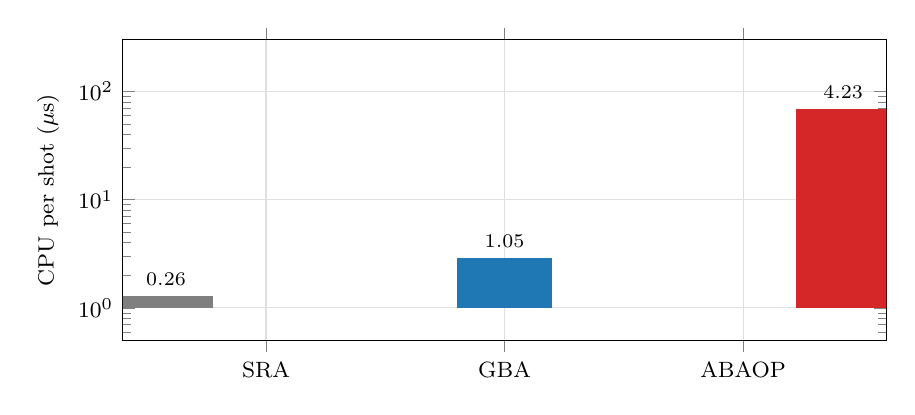
\begin{tikzpicture}
            \begin{axis}[battle, height=5.4cm, ybar, ymode=log, ymin=0.5, ymax=300, xmin=-0.6, xmax=2.6, xtick={0,1,2}, xticklabels={SRA,GBA,ABAOP},
                         ylabel={CPU per shot ($\mu$s)}, bar width=1.2cm, nodes near coords, nodes near coords style={font=\scriptsize}]
                \addplot[fill=cSRA,   draw=none] coordinates {(0,1.30)};
                \addplot[fill=cGBA,   draw=none] coordinates {(1,2.87)};
                \addplot[fill=cABAOP, draw=none] coordinates {(2,68.58)};
            \end{axis}
        \end{tikzpicture}
        \captionof{figure}{CPU time per shot of each agent (logarithmic scale).}
        \label{fig:cpu}
    \end{minipage}
\end{center}

\textbf{Complexity analysis.} To explain these numbers we count the work done to decide and register one shot, using the usual asymptotic notation \cite{cormen2022}. Let $n=10$ be the side of the board, $N=n^2=100$ the number of cells, $F=5$ the number of ships, $S=\sum_i\ell_i=17$ the total length of the fleet, and $M\le N$ the number of shots of a game.

\textbf{SRA.} Choosing the cell is a random index in the list of cells not shot yet: $O(1)$. Registering the shot has two costs: to look for the cell in the list and to remove it (the elements after it move one position), both $O(|U|)$ with $|U|\le N$ (in our games the list had on average 52.6 cells when a shot was made), plus the check of the hit and of the sunk ships, $O(F)=O(1)$. Therefore one shot costs $O(N)$ and a game of $M\le N$ shots costs
\begin{equation}
    T_{\text{SRA}}(N)=\sum_{t=1}^{M}O(N-t)=O(N^2).
\end{equation}
If the list were replaced by one in which the chosen cell is swapped with the last one, a shot would cost $O(1)$ and the game $O(N)$.

\textbf{GBA.} In hunt mode the agent chooses a random cell of the parity list (32.1 cells on average) and removes it, $O(N/p)$. In target mode it tests at most four neighbours, each one $O(1)$ thanks to the coordinate maps, and removes the shot from the list. Every time a ship is sunk (exactly $F=5$ times per game) \texttt{recalc} rebuilds the parity list, that scans about $N/p$ cells each one with an $O(F)$ check, restarts the decision grid ($O(N)$) and looks for an unresolved hit in the whole board ($O(N)$). In the worst case, the ``safety net'' repeats that search once for every hit ($S$ times). Adding all,
\begin{equation}
    T_{\text{GBA}}(N)=\underbrace{M\cdot O(N/p)}_{\text{shots}}+\underbrace{(F+S)\cdot O(N)}_{\text{recalc, safety net}}=O(N^2),
\end{equation}
where the second term is $O(N)$ for a fixed fleet and the first can also be made $O(M)$ with the same trick as for the SRA. So the GBA is $O(N)$ in decisions and $O(N^2)$ as implemented, like the SRA, with a slightly larger constant.

\textbf{ABAOP.} Before every shot the agent builds the density map from zero. For each ship afloat $i$, for each of the two orientations and for each of the $N$ possible positions of its first cell, it examines up to $\ell_i$ cells to decide if the placement is legal (it stops at the first blocked cell) and, if it is, it adds the weight to those $\ell_i$ cells. That is at most $2N\ell_i$ examinations per ship, so
\begin{equation}
    C_{\text{density}}\le\sum_{i\in\mathcal F}2N\ell_i=2NS_{\text{afloat}}\le 2NS=3\,400 \text{ examinations},
\end{equation}
where $S_{\text{afloat}}$ is the total length of the ships that are still afloat. To this we add the search of the maximum ($O(N)$) and of the unresolved hits ($O(N)$), which are negligible against the density. One shot costs $\Theta(NS)$ and a game
\begin{equation}
    T_{\text{ABAOP}}(N)=\sum_{t=1}^{M}\Theta(NS_t)=O(M\,N\,S)=O(N^2S).
\end{equation}
We measured it by counting the examinations in instrumented runs of the program: the first shot of a game on an empty board makes 3\,180 (the bound is 3\,400), and the average over complete games is 1\,449 per shot (44.6 shots per game), which is lower because the ships that sink stop contributing and the blocked cells cut the scans.

\begin{table}[H]
    \centering
    \small
    \renewcommand{\arraystretch}{1.5}
    \resizebox{\linewidth}{!}{\begin{tabular}{|c|p{2.9cm}|c|c|p{3.6cm}|c|}
        \hline
        \rowcolor{blue!20}
        Agent & Work per shot (decision) & Game (decisions) & Game (as implemented) & Basic operations per shot (measured) & CPU per shot \\ \hline
        SRA   & $O(1)$          & $O(N)$   & $O(N^2)$   & $\approx 53$ list positions & 1.30\,$\mu$s \\ \hline
        GBA   & $O(1)$, $O(N)$ per sunk ship & $O(N)$   & $O(N^2)$   & $\approx 32$ list positions + 5 recalculations & 2.87\,$\mu$s \\ \hline
        ABAOP & $\Theta(N\,S)$  & $O(N^2S)$ & $O(N^2S)$  & $\approx 1\,449$ cell examinations & 68.58\,$\mu$s \\ \hline
    \end{tabular}}
    \caption{Complexity of the three agents in terms of the number of cells $N$ and the total length of the fleet $S$, and the counts and times measured in the experiments.}
    \label{tab:complexity}
\end{table}

\textbf{Reading of the analysis.} As implemented, the three agents are quadratic in the number of cells of the board, $O(N^2)=O(n^4)$; what separates them is the constant, and here it is huge: the ABAOP does about $1\,449/52.6\approx28$ times more elementary operations per shot than the SRA, and each of them is more expensive than moving an element of a list, which is consistent with the measured 53 times (Table~\ref{tab:cpu}). Without the inefficiency of the list, the SRA and the GBA would be linear in $N$, and the ABAOP would keep its $O(N^2S)$: it is the only agent whose cost depends on the size of the fleet ($S$) and grows quickly with the size of the board, since one shot costs $\Theta(n^2S)$. The measured CPU time per shot is proportional to the number of shots in a game (the regression of the CPU time on the number of shots gives $1.30$, $2.83$ and $67.3$ microseconds per shot for the SRA, GBA and ABAOP), which also shows that our per-shot model is adequate. A last observation is that for the ABAOP the correlation between CPU time and number of shots is only $0.26$ (for the SRA and GBA it is $0.03$--$0.04$): its cost per shot decreases during the game (fewer ships afloat and more blocked cells), so a long game is not proportionally more expensive.

\end{Resultados}

%%%%%%%%%%%%%%%%%%%%%%%%%%%%%%%%%%%%%%%%%%%%%%%%
\section{Conclusions}
\label{sec:conclusions}

We designed and implemented three agents for Battleship, built a web application to play with them and to observe their decisions, and analysed 70\,000 simulated games. Table~\ref{tab:summary} summarises the result, and the following subsections answer the questions we asked ourselves at the beginning.

\begin{table}[H]
    \centering
    \renewcommand{\arraystretch}{1.4}
    \begin{tabular}{|c|c|c|c|p{4.2cm}|c|}
        \hline
        \rowcolor{blue!20}
        Agent & Shots (mean $\pm$ sd) & Median & Hit rate & Wins against the other kinds & CPU per shot \\ \hline
        SRA   & $95.38\pm4.84$ & 97 & 17.9\,\% & 1 of 20\,000 & 1.30\,$\mu$s \\ \hline
        GBA   & $50.29\pm8.67$ & 51 & 35.0\,\% & 99.99\,\% vs SRA; 33.0\,\% vs ABAOP & 2.87\,$\mu$s \\ \hline
        ABAOP & $44.71\pm9.19$ & 44 & 39.7\,\% & 100\,\% vs SRA; 67.0\,\% vs GBA & 68.58\,$\mu$s \\ \hline
    \end{tabular}
    \caption{Summary of the results of the three agents.}
    \label{tab:summary}
\end{table}

\subsection{Which agent is better?}

Considering the number of shots, which is the performance measure of the problem, the order is clear and statistically solid: ABAOP ($44.71$ shots) $>$ GBA ($50.29$) $\gg$ SRA ($95.38$). The GBA saves 47\,\% of the shots of the SRA and the ABAOP saves 53\,\%. In direct contests the two intelligent agents beat the SRA in practically all the games (9\,999 of 10\,000 and 10\,000 of 10\,000), and the ABAOP beats the GBA in 67.0\,\% of the games (interval 66.1--67.9\,\%), with a mean difference of $5.36\pm0.24$ shots per game.
So the ABAOP is the best agent overall. The difference with the GBA is real but small compared with the variability of a single game (effect size $d_z=0.43$), which means that the better agent still loses one of every three games: in a single game of Battleship luck is still important.
Our results are in agreement with what is known from the references: the median of the SRA is 97 shots as in \cite{berry2011,schwartz2022}; the ABAOP has a median of 44 shots against the 42 reported in \cite{berry2011}, and even the maximum of 73 shots is the same reported there; and our GBA, whose median is 51, is better than the 64 shots reported for the hunt/target strategy with parity, because it follows the line of the ship instead of walking around every hit. We did not investigate the two-shot gap of the ABAOP, but there are several differences of detail that could explain it (weights of the hits, tie-break, information available after a ship is sunk), so we do not claim that our ABAOP is identical to the reference one.

\subsection{Is it worth using the ABAOP, taking the complexity into account?}

The ABAOP costs 68.6 microseconds per shot, 53 times more than the SRA and 24 times more than the GBA, and its work per shot grows with the number of cells and with the length of the fleet ($\Theta(NS)$, against $O(1)$ decisions for the other two). Nevertheless, in absolute terms the cost is small for a $10\times10$ board: 3.07 ms per complete game, so a person never notices it and 10\,000 games are simulated in about a minute.
The relation between cost and benefit shows diminishing returns. The step from the SRA to the GBA saves 45.1 shots per game for an extra $0.02$ ms of CPU (about 0.5 microseconds per shot saved). The step from the GBA to the ABAOP saves 5.6 more shots for an extra 2.9 ms, that is about 520 microseconds per shot saved, roughly a thousand times more per shot saved.
Our answer is therefore: \emph{yes}, it is worth it when the objective is to play as well as possible on a board of this size, because a saving of 11\,\% of the shots becomes a 67\,\% win rate against the GBA and the cost is negligible; but the GBA is the best balance between quality and cost, and it would be the reasonable choice if the board or the fleet were much larger, if the decisions had to be taken thousands of times per second, or if energy consumption (a phone) mattered. A further point in favour of the ABAOP is that it does not need hand-made rules such as the parity or the order of the directions: its behaviour emerges from a single formula, and that would make it easier to adapt to other rules. Its computational cost could be reduced by updating the density map only around the last shot instead of recomputing it from zero, which we did not implement.

\subsection{What the number of shots and the games completed say}

All the 70\,000 games were completed without errors, and in every one both agents sank their whole fleet within 100 shots; the internal consistency checks were satisfied in 100\,\% of the records and the SRA agrees with its closed-form distribution ($p=0.68$), so we trust the simulator and the data.
The SRA needs practically the whole board: 95.4 shots on average, and the 100 shots in 17.1\,\% of its games, so it is useful only as a baseline. When its opponent finishes, it has sunk on average 0.65 (against the GBA) and 0.46 (against the ABAOP) of its five ships.
The GBA and the ABAOP never needed more than 77 and 73 shots, respectively, which gives a guarantee of performance that the SRA does not have; on the other hand, their results are more dispersed (coefficient of variation of 17\,\% and 21\,\% against 5\,\%), because their good games are very good and their bad games are still bad.
Since the result of a game depends on the layout and on luck, a single game says almost nothing: with 100 games the interval of the difference between GBA and ABAOP is still $\pm2.4$ shots, and it takes about 1\,000 games to know it with a precision better than one shot.

\subsection{What the rest of the statistics say}

\begin{itemize}
    \item \textbf{Agents of the same kind} win 50\,\% of the games each ($49.2$ to $49.9\,\%$, all intervals contain 50\,\%), so the experiment has no bias between the left and the right side. The apparent ``draw'' is really a symmetric race in which 3\,\% to 10\,\% of the games are decided by the first shooter, since both agents needed the same number of shots.
    \item \textbf{First-shooter advantage.} It is not a matter of luck but of ties, and it follows Eq.~\eqref{eq:firstmover}: it is the largest for the SRA (about 54\,\% for the first shooter) and disappears when the agents are very different. Alternating the first shooter is therefore necessary to compare agents fairly.
    \item \textbf{Hit rate and first hit.} The ABAOP converts 39.7\,\% of its shots into hits against 35.0\,\% for the GBA and 17.9\,\% for the SRA; and it finds its first hit earlier (shot 4.1 against 5.4 and 5.6), thanks to the density map that sends it to the centre of the board.
    \item \textbf{Sinking times.} The advantage of the ABAOP over the GBA is built between the second and the fourth ship, and it is not increased in the last one, where both must search the same empty area. That is the point of the game where a better strategy would be more valuable.
    \item \textbf{Layout.} It has no influence on the SRA, has a small one on the GBA ($\rho=0.07$) and an important one on the ABAOP ($\rho=0.29$); using the same layout for both agents reduces the variance of the comparison by 29\,\% in the mirror contest of the ABAOP.
\end{itemize}

\subsection{Other aspects}

The experience produced several lessons. First, the design of the experiment is as important as the agents: without the play-out of the loser the shot counts would have been biased, without the alternation of the first shooter the win rates would have been biased, and without the same layout the comparison would have been noisier for the ABAOP. Second, validating the simulator against a closed form (the SRA) gave us confidence to interpret the differences of the other agents. Third, a good visualisation (the decision grids) was very useful to find errors in the agents during their development.
Among the limitations, the model is a race and not a duel, the agents use the information of the ship that has sunk in a way that a human may not have, the board and the fleet are fixed, the density counts each ship independently, and the timer of the browser only has a resolution of 1 ms.
As future work we propose: to sample complete layouts that are consistent with all the observations (a Monte Carlo estimate of the true probability of each cell, instead of the counting of placements), to look one shot ahead instead of being greedy, to update the density incrementally to reduce its cost, to study other board sizes and fleets to check the growth of the cost predicted by the complexity analysis, to compare against a learning agent trained by reinforcement, and to play the agents against each other in the real two-player game where the placement of the fleet can also be optimised.

%%%%%%%%%%%%%%%%%%%%%%%%%%%%%%%%%%%%%%%%%%%%%%%%
%% NOTE: web items are cited in IEEE format; edit the ``Accessed'' dates to the days on which the group really consulted them.
\begin{thebibliography}{99}
    \bibitem{berry2011} N. Berry, ``Battleship,'' \textit{DataGenetics}, Dec. 3, 2011. [Online]. Available: \url{https://www.datagenetics.com/blog/december32011/}. [Accessed: Sep. 21, 2026].
    \bibitem{schwartz2022} A. Schwartz, ``Coding an intelligent Battleship agent,'' \textit{Towards Data Science}, Medium, Apr. 2022. [Online]. Available: \url{https://medium.com/data-science/coding-an-intelligent-battleship-agent-bf0064a4b319}. [Accessed: Sep. 21, 2026].
    \bibitem{vsauce2019} Vsauce2, ``The Battleship algorithm,'' YouTube, Aug. 12, 2019. [Video]. Available: \url{https://www.youtube.com/watch?v=LbALFZoRrw8}. [Accessed: Sep. 21, 2026].
    \bibitem{russell2021} S. Russell and P. Norvig, \textit{Artificial Intelligence: A Modern Approach}, 4th ed. Hoboken, NJ, USA: Pearson, 2021.
    \bibitem{schwartzgit} A. Schwartz, ``Battleship-AI,'' GitHub repository. [Online]. Available: \url{https://github.com/aydinschwa/Battleship-AI}. [Accessed: Sep. 21, 2026].
    \bibitem{waytoosimple2024} Way Too Simple, ``How to win Battleship every time,'' YouTube, Nov. 14, 2024. [Video]. Available: \url{https://www.youtube.com/watch?v=395D3dkts3s}. [Accessed: Sep. 21, 2026].
    \bibitem{always2023} ``How to `always' win at Battleship?'' YouTube, Sep. 10, 2023. [Video]. Available: \url{https://www.youtube.com/watch?v=8FctDuTfcO8}. [Accessed: Sep. 21, 2026].
    \bibitem{mdnloop} Mozilla, ``The event loop,'' \textit{MDN Web Docs}. [Online]. Available: \url{https://developer.mozilla.org/en-US/docs/Web/JavaScript/Event_loop}. [Accessed: Sep. 21, 2026].
    \bibitem{mdnperf} Mozilla, ``Performance: now() method,'' \textit{MDN Web Docs}. [Online]. Available: \url{https://developer.mozilla.org/en-US/docs/Web/API/Performance/now}. [Accessed: Sep. 21, 2026].
    \bibitem{wilson1927} E. B. Wilson, ``Probable inference, the law of succession, and statistical inference,'' \textit{J. Amer. Statist. Assoc.}, vol. 22, no. 158, pp. 209--212, Jun. 1927.
    \bibitem{cormen2022} T. H. Cormen, C. E. Leiserson, R. L. Rivest, and C. Stein, \textit{Introduction to Algorithms}, 4th ed. Cambridge, MA, USA: MIT Press, 2022.
\end{thebibliography}

\end{document}
